% --begin pap's style
\documentclass[handout,10pt]{beamer}

%\usetheme[secheader]{Darmstadt}
%\usetheme{Pittsburgh}

\usepackage[english]{babel}


\usepackage[utf8]{inputenc}
\usepackage[final]{pdfpages}
\usepackage[official]{eurosym}
\usepackage{graphicx}
\usepackage{caption}
\usepackage{csquotes}
\usepackage{multirow}
\usepackage{amsmath}
\usepackage{amsfonts} % for \text
\usepackage{hyperref}
\usepackage{comment}
\usepackage{graphicx}
\usepackage{booktabs}
\usepackage{tabularx}
\usepackage[flushleft]{threeparttable}  % for table notes
\newcommand\mscriptsize[1]{\mbox{\scriptsize\ensuremath{#1}}}
\newcommand\mtiny[1]{\mbox{\tiny\ensuremath{#1}}}

\usepackage{subcaption}

\usepackage[T1]{fontenc}
\usepackage[utf8]{inputenc}
\usepackage{minted}           % core package
\usepackage{xcolor}           % for background color
\definecolor{LightGray}{gray}{0.95}


\definecolor{blueNCS}{rgb}{0.0 0.53 0.74}  
\definecolor{bluepanam}{rgb}{0.0 0.189 0.79} 
\definecolor{Aplgreen}{rgb}{0.55 0.71 0.0}  
\definecolor{greentech}{cmyk}{0.7 0.0 1.0 0.0} 
\definecolor{DarkBlue}{rgb}{0.1,0.1,0.9}

\hypersetup{
    colorlinks=true,
    linkcolor=bluepanam,
    filecolor=bluepanam,      
    urlcolor=bluepanam,
    pdftitle={Overleaf Example},
    pdfpagemode=FullScreen,
    }

\setbeamercolor{palette primary}{bg=white,fg=black}
\setbeamercolor{palette secondary}{bg=white,fg=bluepanam}
\setbeamercolor{palette tertiary}{bg=white,fg=bluepanam}
\setbeamercolor{palette quaternary}{bg=white,fg=bluepanam}
\setbeamercolor{structure}{fg=bluepanam} % itemize, enumerate, etc
\setbeamercolor{section in toc}{fg=bluepanam} % TOC sections


%% \setbeamercolor{section in head/foot}{fg=white, bg=blue}
\setbeamercolor{title}{fg=bluepanam, bg=white}
\setbeamercolor{author}{fg=black, bg=white}
\setbeamercolor{institute}{fg=black, bg=white}
\setbeamercolor{date}{fg=white, bg=white}


\setbeamercolor{section in head/foot}{fg=bluepanam, bg=white}     
     
\setbeamercolor{author in head/foot}{fg=bluepanam, bg=white}
%\setbeamercolor{author in head/foot}{fg=white, bg=white}
\beamertemplatenavigationsymbolsempty
% --end pap's style

%\usepackage[backend=biber,
%            style=apa,
%            block=par,]{biblatex}
%\usepackage[backend=bibtex]{biblatex}
%\bibliography{sample.bib}
%\usepackage{natbib}
%\bibliographystyle{plain}  % or ieeetr, apalike, etc.
%\bibliography{sample_bibtex.bib}

%\newcommand{\customcite}[1]{\citeauthor{#1}, \citetitle{#1}, \citeyear{#1}, \citeurl{#1}}
%\newcommand{\customcitenourl}[1]{\citeauthor{#1}, \citetitle{#1}, \citeyear{#1}}
\newcommand{\parensmall}[1]{{\scriptsize #1}}

%\newcommand{\comment}[1]{}

\title{Natural language processing of subjectivity analysis in personal narratives}
\author{Gustave Cortal}
\titlegraphic{
    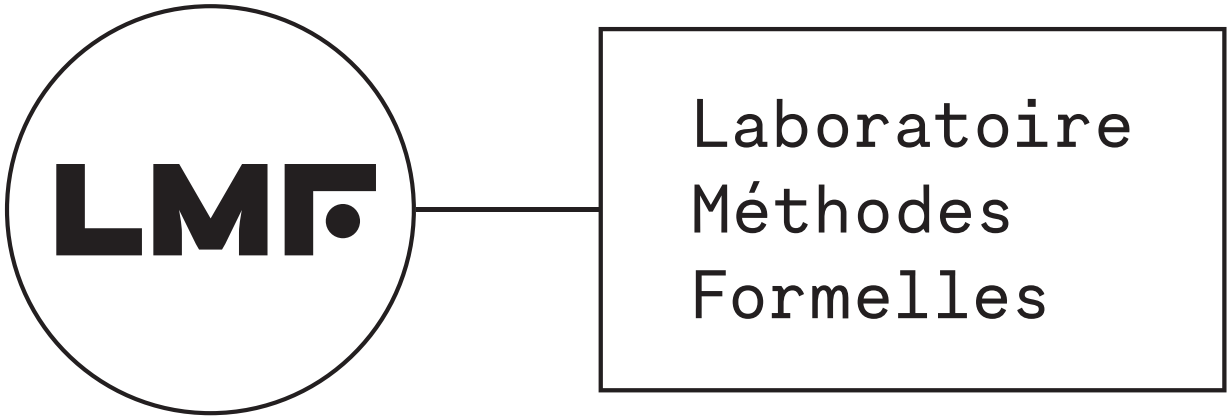
\includegraphics[width=4cm]{img/lmf_logo_emnlp.png}
    \hspace{1cm}
    
\includegraphics[width=5cm]{img/logo_ens_saclay.png}
}
\date{\today}

\makeatletter
\defbeamertemplate*{footline}{myminiframes theme}
  {%
    \begin{beamercolorbox}[colsep=1.5pt]{upper separation line foot}
    \end{beamercolorbox}
    \begin{beamercolorbox}[ht=2.5ex,dp=1.125ex,%
      leftskip=.3cm,rightskip=.3cm plus1fil]{author in head/foot}%
      \leavevmode{\usebeamerfont{author in head/foot}}%
      \hfill%
    %\insertframenumber{}\,/\,\inserttotalframenumber%
    \end{beamercolorbox}%
    \begin{beamercolorbox}[ht=2.5ex,dp=2.125ex,leftskip=.3cm,rightskip=.3cm plus1fil]{section in head/foot}%
      %%      {\usebeamerfont{section in head/foot} somthing written here \hfill  \setlength{\fboxrule}{0pt}\setlength{\fboxsep}{0pt}\fcolorbox{blueNCS}{blueNCS!70}{My own image here}}%
      {\usebeamerfont{section in head/foot} \insertshortauthor \hfill  %\setlength{\fboxrule}{0pt}\setlength{\fboxsep}{0pt}\fcolorbox{blueNCS}{blueNCS!100}{foobar etc}
      }%
      \insertframenumber{}\,/\,\inserttotalframenumber%
    \end{beamercolorbox}%
    \begin{beamercolorbox}[colsep=1.5pt]{lower separation line foot}
    \end{beamercolorbox}
  }
  \makeatother


\begin{document}

\setlength{\parskip}{5pt}%
\setlength{\parsep}{0pt}%
\setlength{\itemsep}{0.25cm}%
\setlength{\leftmargini}{0.5cm}

\begin{frame}
  \titlepage
\end{frame}


\begin{frame}{Introduction}

%\pause

%\textbf{Observation}: The field emphasizes formal and mathematical tasks, whereas social and emotional tasks remains underexplored

%\textbf{Observation}: LLMs have mastered linguistic knowledge but still lack functional skills such as emotional reasoning %The research field focuses more on formal reasoning compared to emotional and social reasoning.
%contastat de these au debut, moins vrai mtn

%\vspace{0.5cm}
\pause

\textbf{Research question}: How to model subjective experience in narratives?


\vspace{0.5cm}
\pause

\textbf{Steps}:

\begin{itemize}[<+->]
    \item Definition of objectives and scope using cognitive science
    \item Construction of an emotion dataset 
    \item Training of language models for emotion analysis 
    \item Formalization of style in narratives 
\end{itemize}

\vspace{0.5cm}
\pause

\small

\textit{Each step lead to a first-author article in an international conference} %(including EMNLP and LREC-COLING)

%\textit{My research models are publicly hosted on Hugging Face and were trained using the Jean Zay supercomputer}
    
\end{frame}

\begin{frame}{Definition of objectives and scope using cognitive science}

\textbf{Goal}: Identify limitations and research directions

\pause
\vspace{0.5cm}

I review psychological theories of emotion and emotion annotation schemes in NLP

\pause
\vspace{0.5cm}

What are current \textbf{limitations}? 

\begin{itemize}[<+->]
    \item Different emotion theories lead to divergences in how to annotate them in the text
    \item Some linguistic and cognitive science theories are not considered
    \item There is no benchmark that evaluates the richness of the emotional phenomenon
\end{itemize}


\vspace{0.5cm}

\scriptsize

\textbf{G. Cortal} and C. Bonard. \href{https://aclanthology.org/2024.cmcl-1.23/}{Improving Language Models for Emotion Analysis: Insights from Cognitive Science}. \textit{CMCL, ACL 2024}.
    
\end{frame}

\begin{frame}{Definition of objectives and scope using cognitive science}

How to integrate psychological theories of emotion?

\pause
\vspace{0.5cm}

I use the \textbf{integrated framework for emotion theories} (Scherer, 2022):

\begin{figure}
    \centering
    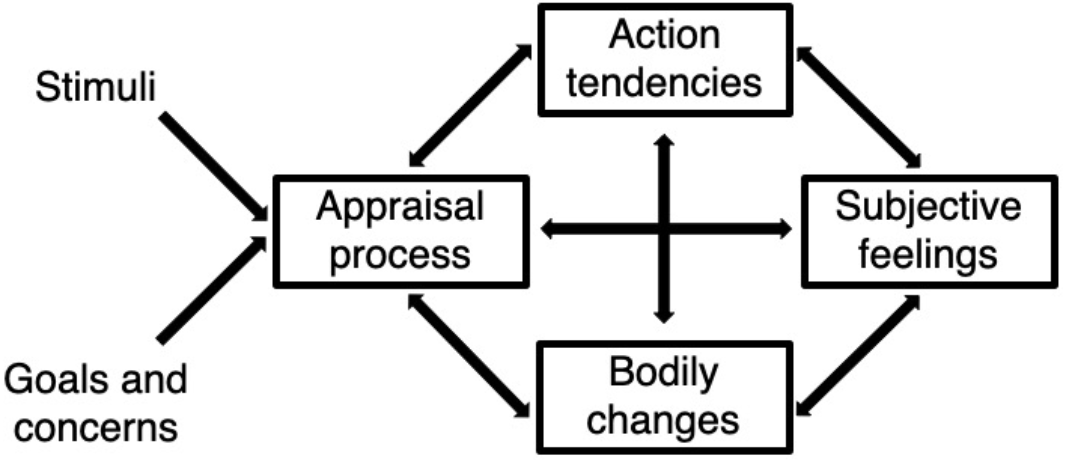
\includegraphics[width=0.8\linewidth]{img/scherer_integrated_framework.png}
    \caption{Emotional episodes are synchronized changes in four components.}
    \label{fig:placeholder}
\end{figure}
    
\end{frame}

\begin{frame}{Definition of objectives and scope using cognitive science}

Which verbal signs are used to infer expressed emotions?

\pause
\vspace{0.5cm}

Raphaël Micheli categorizes a range of linguistic markers into three \textbf{emotion expression modes} (Micheli, 2014). The emotion can be: 

%\cite{Micheli2014}
\pause
\vspace{0.5cm}

\begin{itemize}[<+->]
    \item \textit{labeled} explicitly with an emotional term ("I am \underline{sad}")
    \item \textit{shown} with utterance features such as interjections and punctuations ("\underline{Ah!} That's great\underline{!}")
    \item \textit{suggested} with the description of a situation which generally, in a given sociocultural context, leads to an emotion ("\underline{She gave me a gift}")
\end{itemize}

\pause
\vspace{0.5cm}

$\rightarrow$ Different emotion expression modes are more or less difficult to interpret.
\end{frame}

\begin{frame}{Construction of an emotion dataset}

\textbf{Goal}: A more comprehensive understanding of emotional events

\pause

\begin{table}
    \centering
    \resizebox{0.9\textwidth}{!}{
\begin{tabular}{l|p{0.78\textwidth}}
 
                   \textbf{Component} &
                 \textbf{Answer} \\
 
\hline
          \textsc{behavior} & I'm giving a lecture on a Friday morning at 8:30. A student goes out and comes back a few moments later with a coffee in his hand. \\
\textsc{feeling} & My heart is beating fast, and I freeze, waiting to know how to act. \\
  \textsc{thinking} & I think this student is disrupting my class. \\
\textsc{territory} & The student attacks my ability to be respected in class. \\
 
\end{tabular}}
%\captionof{table}{Example of an emotional narrative structured according to emotion components. More than 1,000 narratives were collected using emotion regulation questionnaires.}
\label{tab:description_corpus}
\end{table} % open-ended questions, my thesis director and I

\small
More than 1,000 narratives were collected during emotion regulation sessions
\vspace{0.5cm}

\scriptsize

\textbf{G. Cortal}, A. Finkel, P. Paroubek, L. Ye. \href{https://aclanthology.org/2023.latechclfl-1.8/}{Emotion Recognition based on Psychological Components in Guided Narratives for Emotion Regulation}. \textit{SIGHUM, EACL 2023}.% \href{https://underline.io/lecture/71953-emotion-recognition-based-on-psychological-components-in-guided-narratives-for-emotion-regulation}{video}.
    
\end{frame}

\begin{frame}{Training language models for emotion analysis}

\textbf{Goal}: Discrete emotion detection based on components

\vspace{0.5cm}
\pause

\begin{table}
    \centering
    \resizebox{0.9\textwidth}{!}{
\begin{tabular}{l|lllllll}

&\multicolumn{3}{c}{\textbf{Logistic Regression}}&\multicolumn{3}{c}{\textbf{CamemBERT}} \\

                   \textbf{Component} &  Precision &     Recall &   $F_1$ &  Precision &     Recall &   $F_1$ \\
\hline
              All  & 71.2\,\mscriptsize{(2.6)} & 69.1\,\mscriptsize{(2.2)} & 67.8\,\mscriptsize{(2.3)} & \textbf{85.1} & \textbf{84.8} & \textbf{84.7} \\
              Without \textsc{behavior}   & 77.4\,\mscriptsize{(2.3)} & 75.8\,\mscriptsize{(2.4)} & 74.5\,\mscriptsize{(2.6)} & 80.3 & 79.8 & 79.7 \\
              Without \textsc{feeling}  & 64.3\,\mscriptsize{(1.9)} & 61.5\,\mscriptsize{(1.2)} & 61.3\,\mscriptsize{(2.2)} & 81.6 & 79.8 & 79.9  \\
              Without \textsc{thinking}  & 70.9\,\mscriptsize{(1.8)} & 69.1\,\mscriptsize{(2.0)} & 68.3\,\mscriptsize{(2.2)} & 79.6 & 78.5 & 78.7 \\
              Without \textsc{territory}  & 64.3\,\mscriptsize{(4.1)} & 64.5\,\mscriptsize{(2.4)} & 62.3\,\mscriptsize{(2.8)} & 78.7 & 78.5 & 78.6 \\
          Only \textsc{behavior}  & 52.1\,\mscriptsize{(3.5)} & 54.6\,\mscriptsize{(2.9)} & 51.7\,\mscriptsize{(2.9)} & 68.4  & 67.1 & 66.6 \\
Only \textsc{feeling}  & 69.6\,\mscriptsize{(1.5)} & 68.9\,\mscriptsize{(2.1)} & 68.4\,\mscriptsize{(2.0)} & 67.8 & 68.4 & 67.7 \\
  Only \textsc{thinking}  & 50.1\,\mscriptsize{(3.4)} & 53.8\,\mscriptsize{(2.3)} & 50.6\,\mscriptsize{(2.7)} & 70.5 & 70.1 & 70.1 \\
              Only \textsc{territory}  & 68.2\,\mscriptsize{(1.8)} & 66.8\,\mscriptsize{(2.2)} & 66.6\,\mscriptsize{(2.3)} & 71.4 & 68.4 & 68.9 \\
\end{tabular}}
    %\caption{Scores (± std) for discrete emotion classification based on components.}
    \label{tab:pred_emotion}
\end{table}

\vspace{0.5cm}

\scriptsize

\textbf{G. Cortal}, A. Finkel, P. Paroubek, L. Ye. \href{https://aclanthology.org/2023.latechclfl-1.8/}{Emotion Recognition based on Psychological Components in Guided Narratives for Emotion Regulation}. \textit{SIGHUM, EACL 2023}.
    
\end{frame}

\begin{frame}{Training language models for emotion analysis}

Need other datasets with narrative structure, emotional content, and available for research

\vspace{0.5cm}
\pause

Quantitative dream analysis examines recurring patterns between narrative elements using a database of dream narratives and an annotation scheme (Domhoff, 2004)

\vspace{0.5cm}
\pause

The annotation process is complex and costly

\vspace{0.5cm}
\pause

How to automate the annotation process?

%side project in my PhD
    
\end{frame}

\begin{frame}{Training language models for emotion analysis}

\textbf{Goal}: Character and emotion detection in dream narratives

\pause

\begin{figure}
    \centering
    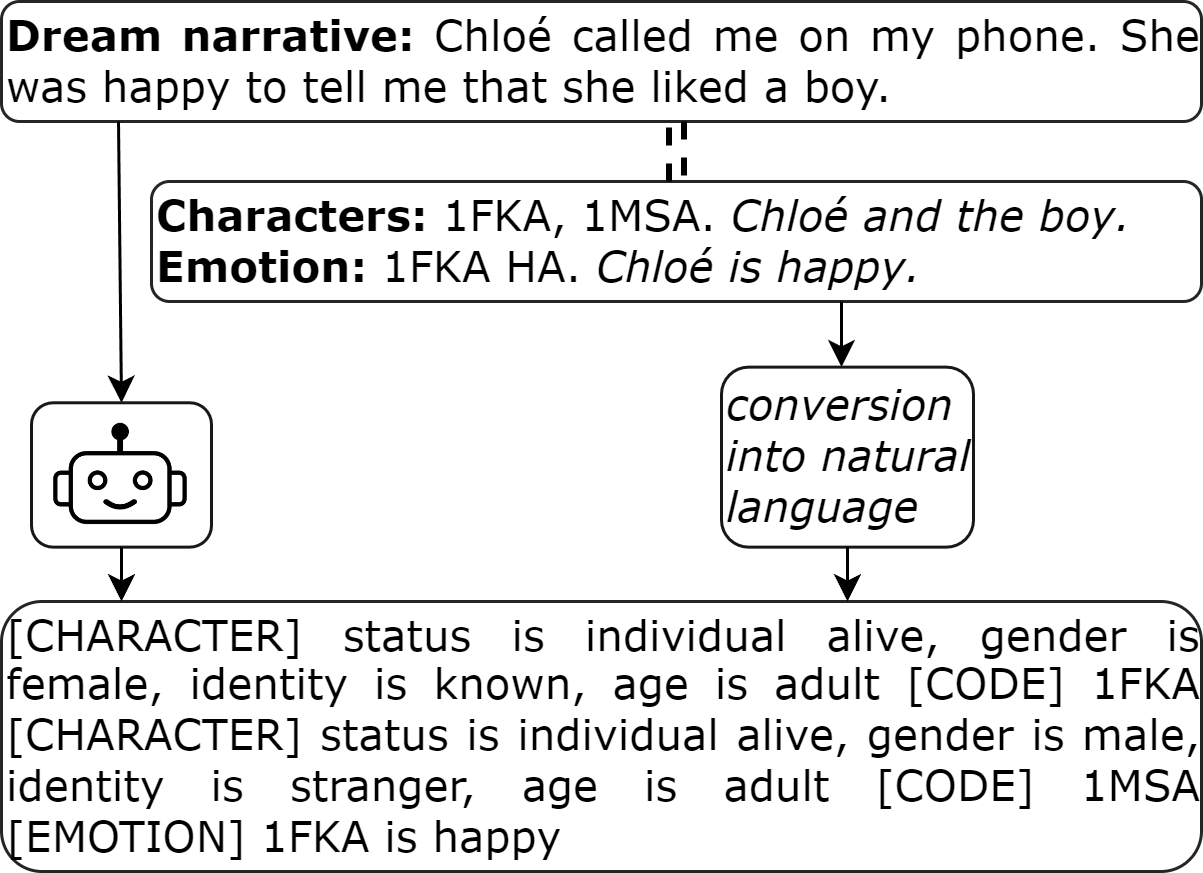
\includegraphics[width=0.6\linewidth]{img/dream_method.png}
    %\caption{Codes describing characters and their emotions are converted into
%natural language to produce the training data.}
    \label{fig:placeholder}
\end{figure}

\scriptsize

\textbf{G. Cortal}. \href{https://aclanthology.org/2024.lrec-main.1282/}{Sequence-to-Sequence Language Models for Character and Emotion Detection in Dream Narratives}. \textit{LREC-COLING 2024}.
    
\end{frame}

\begin{frame}{Training language models for emotion analysis}

\scriptsize

LaMini-Flan-T5 finetuned on 1823 dream narratives

\small

\begin{table}
    \centering
    \resizebox{0.9\textwidth}{!}{
\begin{tabular}{l|cccccc}
\textbf{Model} & \textbf{Status} & \textbf{Gender} & \textbf{Identity} & \textbf{Age} & \textbf{Character} & \textbf{Emotion} \\
\hline
\textsc{baseline} & 82.87 & 78.02 & 76.17 & 86.21 & 64.74 &  75.13 \\
\hline
\textsc{no\textsubscript{semantics}} & 71.37 & 56.54\textbf{*} & 61.0  & 90.51  & 41.79\textbf{*} &  75.79 \\
\textsc{no\textsubscript{names}} & 80.66\textbf{*}  & 74.32\textbf{**}  & 74.2  & 83.95\textbf{*}  & 60.93\textbf{**} &  73.04\textbf{*} \\
\hline
\textsc{size\textsubscript{small}} & 78.35\textbf{**}  & 72.13\textbf{**}  & 70.25\textbf{**}  & 81.66\textbf{**}  & 56.79\textbf{**} &  70.15\textbf{**} \\
\textsc{size\textsubscript{large}} & 84.51\textbf{*} & 80.3\textbf{**}  & 78.63\textbf{**}  & 87.29  & 67.63\textbf{**} & 74.71 \\
\hline
\textsc{first\textsubscript{group}} & 82.33  & 77.71  & 74.86  & 85.61  & 63.71 &  71.94 \\
\textsc{first\textsubscript{individual}} & 80.59\textbf{**}  & 76.14  & 74.22\textbf{*}  & 83.87\textbf{**} & 62.67 &  67.32 \\
\textsc{first\textsubscript{emotion}} & 83.92 & 78.74 & 77.06  & 87.63  & 64.97 &  72.03 \\
\hline
\textsc{conversion\textsubscript{comma}} & 84.02\textbf{**}  & 79.84\textbf{**}  & 77.67\textbf{**}  & 87.08\textbf{*}  & 66.69\textbf{**} &  73.68 \\
\textsc{conversion\textsubscript{marker}} & 82.39  & 78.45  & 76.53  & 86.09  & 65.44 &  74.36 \\
\hline
\textsc{StableBeluga\textsubscript{1}} &   43.95\textbf{**} &   39.76\textbf{**} &     31.25\textbf{**} &  56.16\textbf{**} &      15.65\textbf{**} & -\\
\textsc{StableBeluga\textsubscript{3}} &   52.44\textbf{**} &   46.49\textbf{**} &     38.46\textbf{**} &  63.88\textbf{**} &      21.06\textbf{**} & -\\
\textsc{StableBeluga\textsubscript{5}} &   55.89\textbf{**} &   46.29\textbf{**} &     42.61\textbf{**} &  63.73\textbf{**} &      24.86\textbf{**} & - \\
\hline
\textsc{cross-validation} & 86.28 & 81.9  & 79.51  & 89.52 & 68.64 &  76.18\\
\end{tabular}}
    \label{tab:result}
\end{table}

\vspace{0.5cm}
\scriptsize

%Generated dream narratives available on \href{https://gustavecortal.com/project/oneirogen}{gustavecortal.com}.

%\href{https://huggingface.co/gustavecortal/oneirogen-7B}{Oneirogen}, a language model for dream generation. 2024.

%\href{https://huggingface.co/gustavecortal/dream-t5}{Dream‑T5}, a language model for emotion and character prediction in dream narratives. 2023.

\textbf{G. Cortal}. \href{https://aclanthology.org/2024.lrec-main.1282/}{Sequence-to-Sequence Language Models for Character and Emotion Detection in Dream Narratives}. \textit{LREC-COLING 2024}.
    
\end{frame}



\begin{frame}{Formalization of style in narratives}

\textit{How} subjective experience is communicated?

\vspace{0.5cm}
\pause

\textbf{Goal}: Formalize style as patterns of linguistic choices that encode subjective experience

\pause
\vspace{0.5cm}

\begin{table}[!ht]
  \centering
  \small
  \renewcommand{\arraystretch}{1.1}
  \begin{threeparttable}
  
    \begin{tabular}{l|l|l}
      \textbf{Clause} & \textbf{Process (code)} & \textbf{Participants} \\
      \midrule
      I wake in a dark room         & Action (\textbf{a})  & Actor \\
      I feel a cold wind            & Mental (\textbf{m})  & Senser,\\
                                            &             & Phenomenon \\
      I tell myself to move         & Verbal (\textbf{v})  & Sayer,\\
                                            &             & Recipient \\
      \bottomrule
    \end{tabular}

    \begin{tablenotes}[flushleft]
      \footnotesize
      \item \textbf{Sequence:} $amv$\quad|\quad
            \textbf{Substrings:} \{am, mv\}
    \end{tablenotes}
  \end{threeparttable}
  \caption{Illustrative pipeline. Each narrative is mapped to a symbolic sequence using an alphabet based on extracted features}
    \label{tab:example}
\end{table}

\scriptsize

\textbf{G. Cortal} and A. Finkel. \href{https://gustavecortal.com/data/Formalizing_Style_in_Personal_Narratives.pdf}{Formalizing Style in Personal Narratives}. \textit{EMNLP 2025}.
    
\end{frame}

%\begin{frame}{Formalization of style in narratives}

%\begin{figure}
%    \centering
%    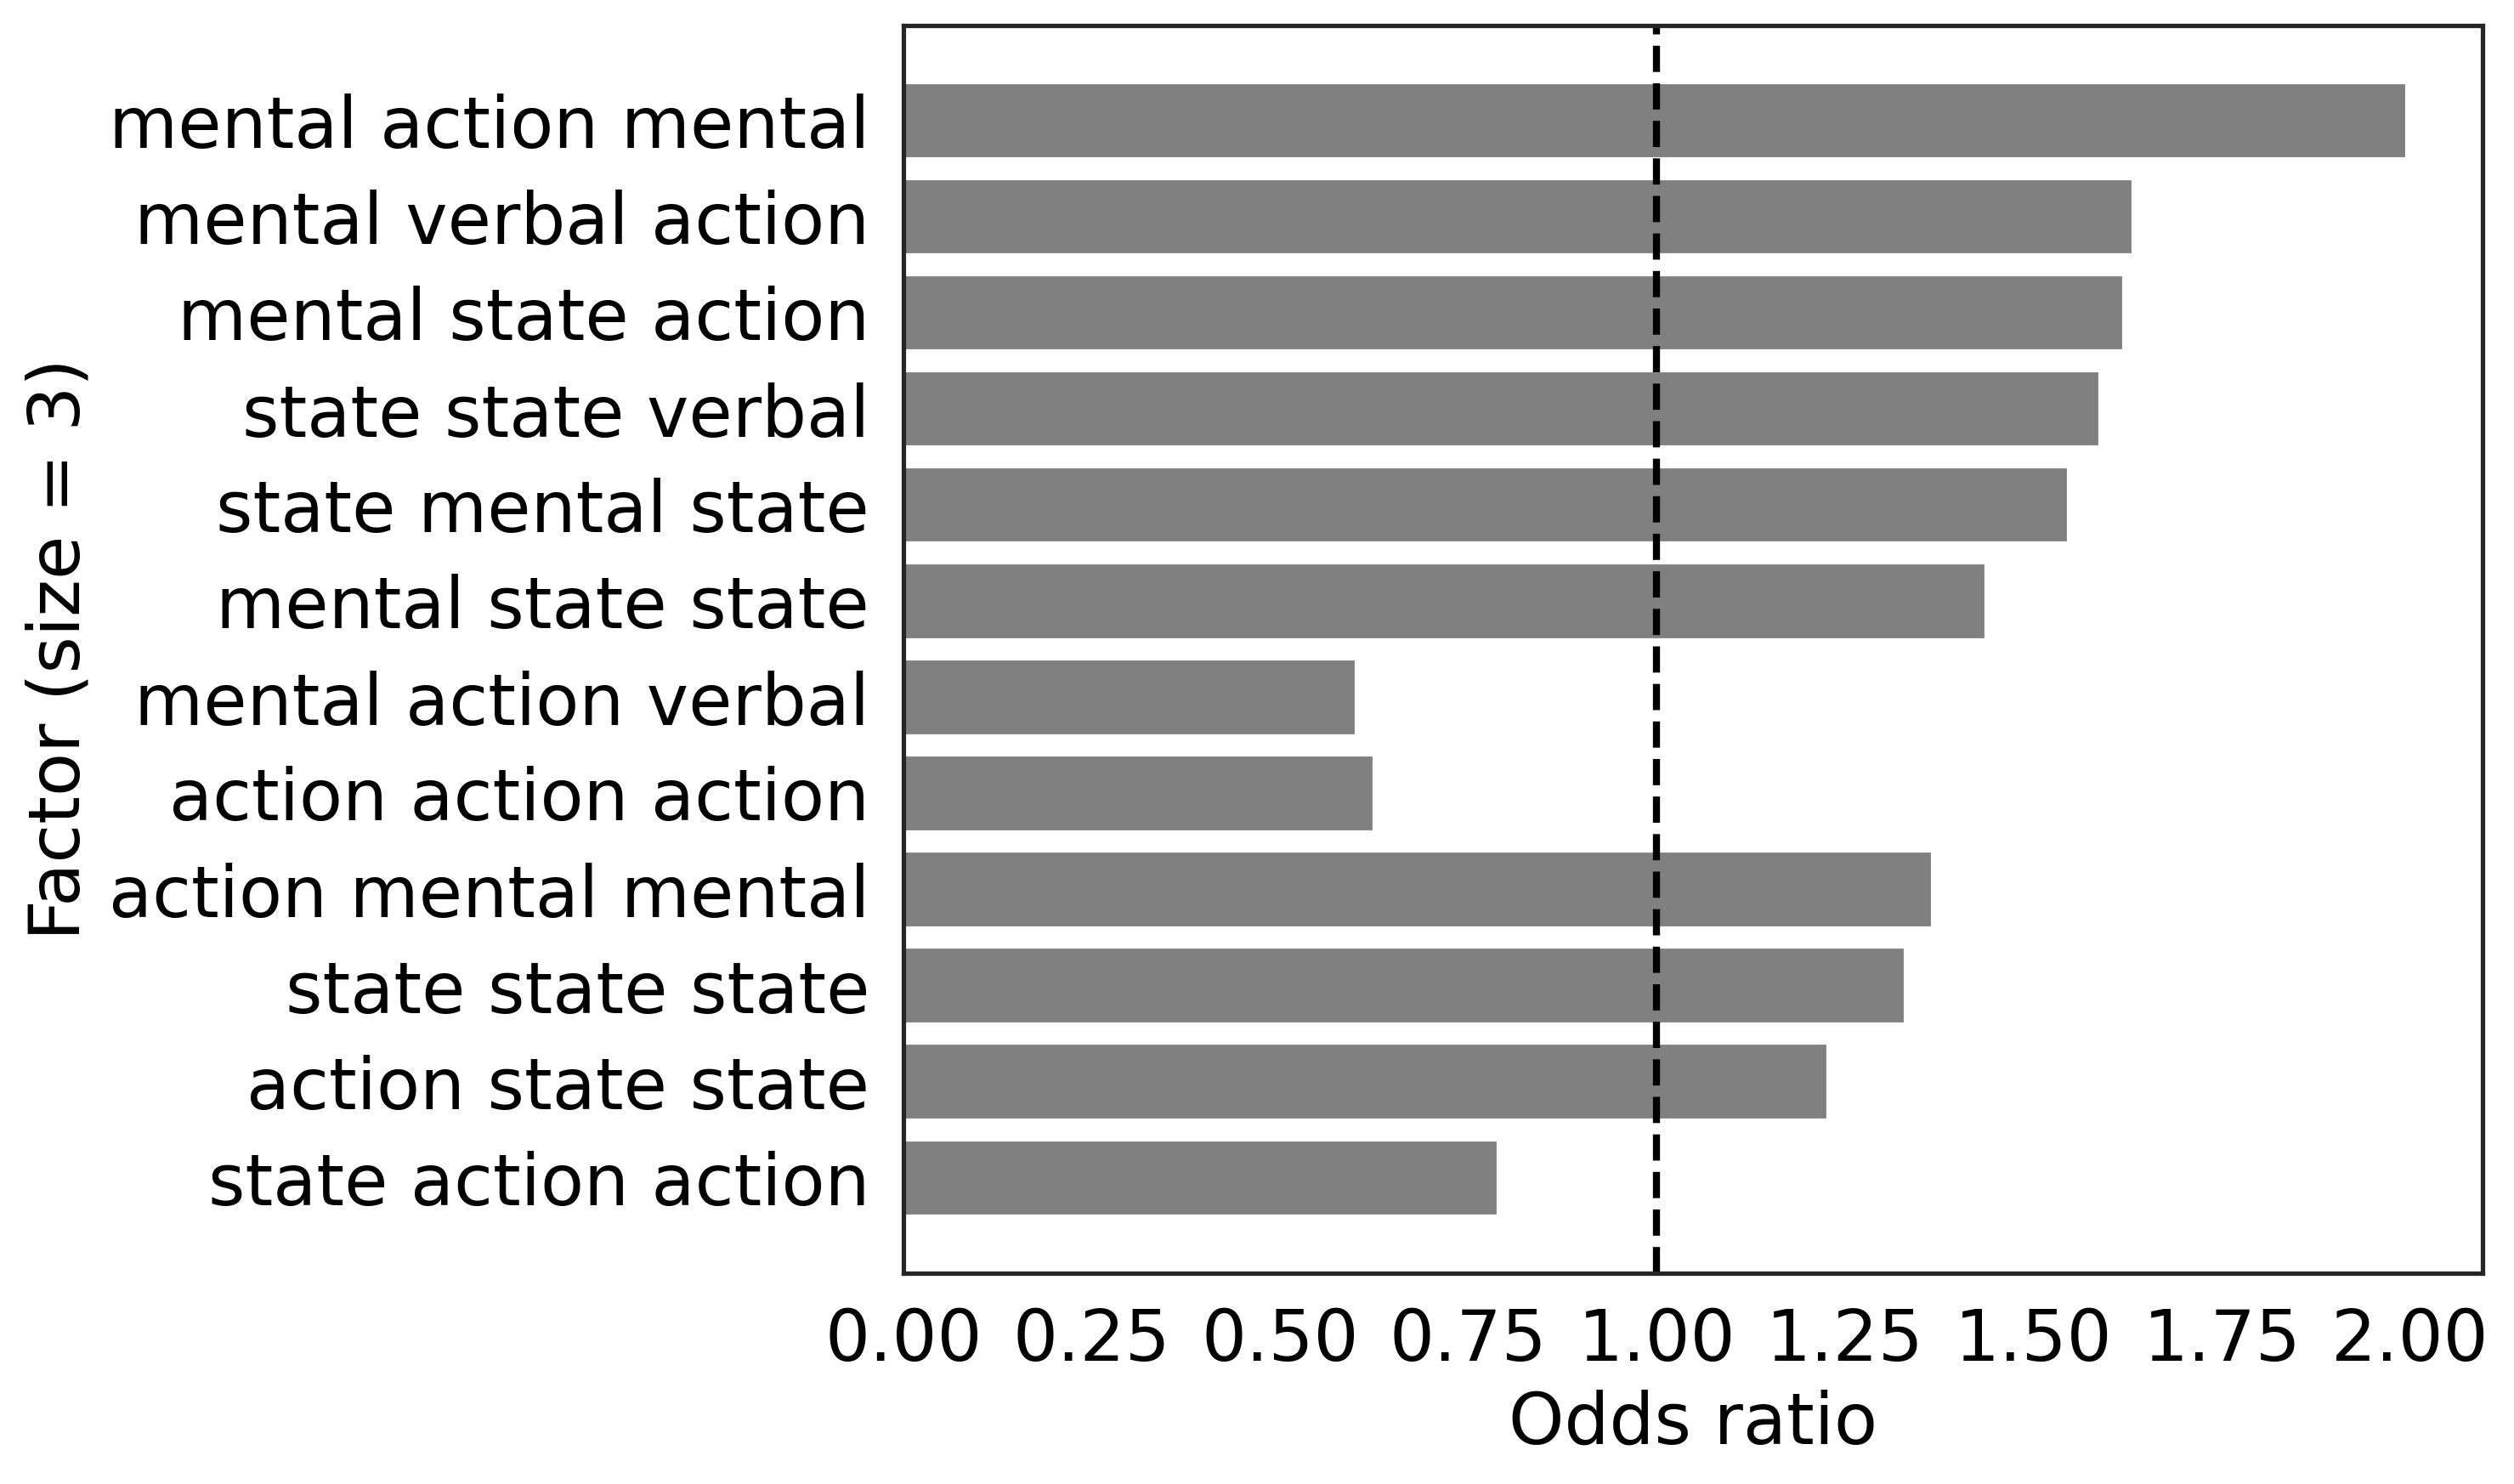
\includegraphics[width=0.8\linewidth]{img/blind_odds_3.png}
%    \caption{Top substring odds ratio between the blind series and the norm. Based on 381 sequences from 15 blind dreamers}
%    \label{fig:placeholder}
%\end{figure}

%\vspace{0.5cm}

%\scriptsize

%\textbf{G. Cortal} and A. Finkel. \href{https://gustavecortal.com/data/Formalizing_Style_in_Personal_Narratives.pdf}{Formalizing Style in Personal Narratives}. \textit{EMNLP 2025}.
    
%\end{frame}

\begin{frame}{Introduction}

\textbf{Research question}: How is subjective experience communicated in narratives?

\vspace{0.5cm}
\pause

We use narratives to express our representations of reality and make sense of the world %(Bruner, 1990) 

\vspace{0.5cm}
\pause

In everyday usage, style refers to a distinctive manner of expression

\vspace{0.5cm}
\pause

We use style as a proxy to study how subjective experience is linguistically communicated

\vspace{0.5cm}
\pause

We narrow the general definition of style: \textit{a distinctive manner of communicating subjective experience in narratives}

\end{frame}

\begin{frame}{Contributions}

\textbf{Problem}: Style is an intuitive notion; we need an operational definition

\vspace{0.25cm}
\pause

\textbf{Hypothesis}: An individual uses some redundant choices of features that characterize its style

\vspace{0.25cm}
\pause

\textbf{Research task}: Formalize style as \textit{patterns of linguistic choices that encode subjective experience}

\vspace{0.5cm}
\pause

\begin{enumerate}[<+->]
    \item A sequence-based framework defining style as patterns in sequences of linguistic choices grounded in systemic functional linguistics
    \item A methodology for automatically identifying patterns using sequence analysis
    \item A case study on dream narratives %, showing how the analysis of patterns can reveal psychological insights
\end{enumerate}
    
\end{frame}

\begin{frame}{Categorizing linguistic features}

Our categorization is grounded in \textit{systemic functional linguistics}: language represents experience through \textit{processes, participants and circumstances}%  (Halliday, 2014)

\pause

\begin{table}[!htb]
    \centering
    \resizebox{\textwidth}{!}{
    \begin{tabular}{p{4cm}|p{11cm}}
        %\hline
        \textbf{Processes} & \textbf{Examples} \\ \hline
        \textit{Action}: actions and events in the physical world. &
        [He]$_{\text{Actor}}$ [\textbf{takes}]$_{\text{Action}}$ [the valuable]$_{\text{Affected}}$ \newline
        
        [Members of my cult]$_{\text{Actor}}$ [\textbf{have made]}$_{\text{Action}}$ [1500 euros]$_{\text{Result}}$ \newline
        
        [I]$_{\text{Actor}}$ [\textbf{give}]$_{\text{Action}}$ [her]$_{\text{Recipient}}$ [a chance]$_{\text{Range}}$ \\ \hline
        
        \textit{Mental}: internal experiences such as thoughts, perceptions, and feelings. &
        [We]$_{\text{Senser}}$ [\textbf{believe}]$_{\text{Mental}}$ [women are the leaders of change]$_{\text{Phenomenon}}$ \newline
        
        [The moon]$_{\text{Senser}}$ [\textbf{sees}]$_{\text{Mental}}$ [the earth]$_{\text{Phenomenon}}$ \newline
        
        [He]$_{\text{Senser}}$ [\textbf{disliked}]$_{\text{Mental}}$ [Gilbert's writing]$_{\text{Phenomenon}}$ \\ \hline
        
        \textit{Verbal}: acts of communication. &
        [David]$_{\text{Sayer}}$ [\textbf{said}]$_{\text{Verbal}}$ [``the corrupt, criminals and money launderers'']$_{\text{Verbiage}}$ \\ \hline
        
        \textit{State}: states of being, having, or existence. &

         There [\textbf{was}]$_{\text{Existential}}$ [a swimming pool]$_{\text{Existent}}$ \newline
        
        [John]$_{\text{Carrier}}$ [\textbf{is}]$_{\text{State}}$ [an interesting teacher]$_{\text{Attribute}}$ \newline
        
        [Hadrian's Wall]$_{\text{Possessor}}$ [\textbf{has}]$_{\text{State}}$ [something for everyone]$_{\text{Possessed}}$ \\ %\hline
    \end{tabular}}
    \caption{Processes with their participants.}
    \label{tab:process_participants}
\end{table}
    
\end{frame}

\begin{frame}{Pipeline for our sequence-based framework}


\begin{table}[!ht]
  \centering
  \small
  \renewcommand{\arraystretch}{1.1}
  \begin{threeparttable}
    %\caption{Illustrative pipeline for our sequence-based framework. We first segment “I wake in a dark room. I feel a cold wind. I tell myself to move.” into clauses, then identify features such as processes and participants for each clause. Each text is mapped to a symbolic sequence using an alphabet based on extracted features.}
    \label{tab:example}
    \begin{tabular}{lll}
      %\toprule
      \textbf{Clause} & \textbf{Process (symbol)} & \textbf{Participants} \\
      \midrule
      I wake in a dark room         & Action (\textbf{a})  & Actor \\
      I feel a cold wind            & Mental (\textbf{m})  & Senser,\\
                                            &             & Phenomenon \\
      I tell myself to move         & Verbal (\textbf{v})  & Sayer,\\
                                            &             & Recipient \\
      \bottomrule
    \end{tabular}

    \begin{tablenotes}[flushleft]
      \footnotesize
      \item \textbf{Sequence:} $amv$\quad|\quad
            \textbf{Substrings:} \{am, mv\}
    \end{tablenotes}
  \end{threeparttable}
\end{table}

\pause

\begin{enumerate}[<+->]
    \item We first segment \textit{“I wake in a dark room. I feel a cold wind. I tell myself to move.”} into clauses
    \item Identify features (\textit{e.g.}, processes and participants) for each clause
    \item Each narrative is mapped to a symbolic sequence using an alphabet based on identified features
\end{enumerate}

%We define \textit{style} as patterns in choices within a system of linguistic features inspired by the transitivity system in systemic functional linguistics. We now need to explain what is a choice. To account for a subjective experience, an author makes a series of choices within a system of features. 
    
\end{frame}

\begin{frame}{Case Study on Dream Narratives}

We apply our framework to dream narratives as they possess a narrative structure and represent attempts to communicate subjective experience

\vspace{0.25cm}
\pause

We use DreamBank, a database of more than 27,000 narratives with 72 series of dreamers

\vspace{0.25cm}
\pause

We analyze five series of dreamers: long-term blind dreamers (n=361), \textit{ed} (a widower, n=139), \textit{izzy} (a teenager, n=1091), \textit{merri} (an artist, n=202), and \textit{viet} (a Vietnam War veteran with PTSD, n=566)%. A description of each series is accessible on the DreamBank

\vspace{0.25cm}
\pause

We construct a \textit{norm} (n=720) to compare how each series deviates from a hypothetical average dreamer %This norm comprises a random sample of ten narratives from each series of DreamBank, resulting in a collection of 720 dream narratives.


\vspace{0.25cm}
\pause

To identified features, we perform in-context learning with Llama 3 8B
    
\end{frame}

\begin{frame}{Results on the Vietnam War veteran}

We compare the proportion of sequences containing a given substring

\pause

\begin{figure}[!htb]
     \begin{subfigure}[b]{0.5\textwidth}
         \centering
         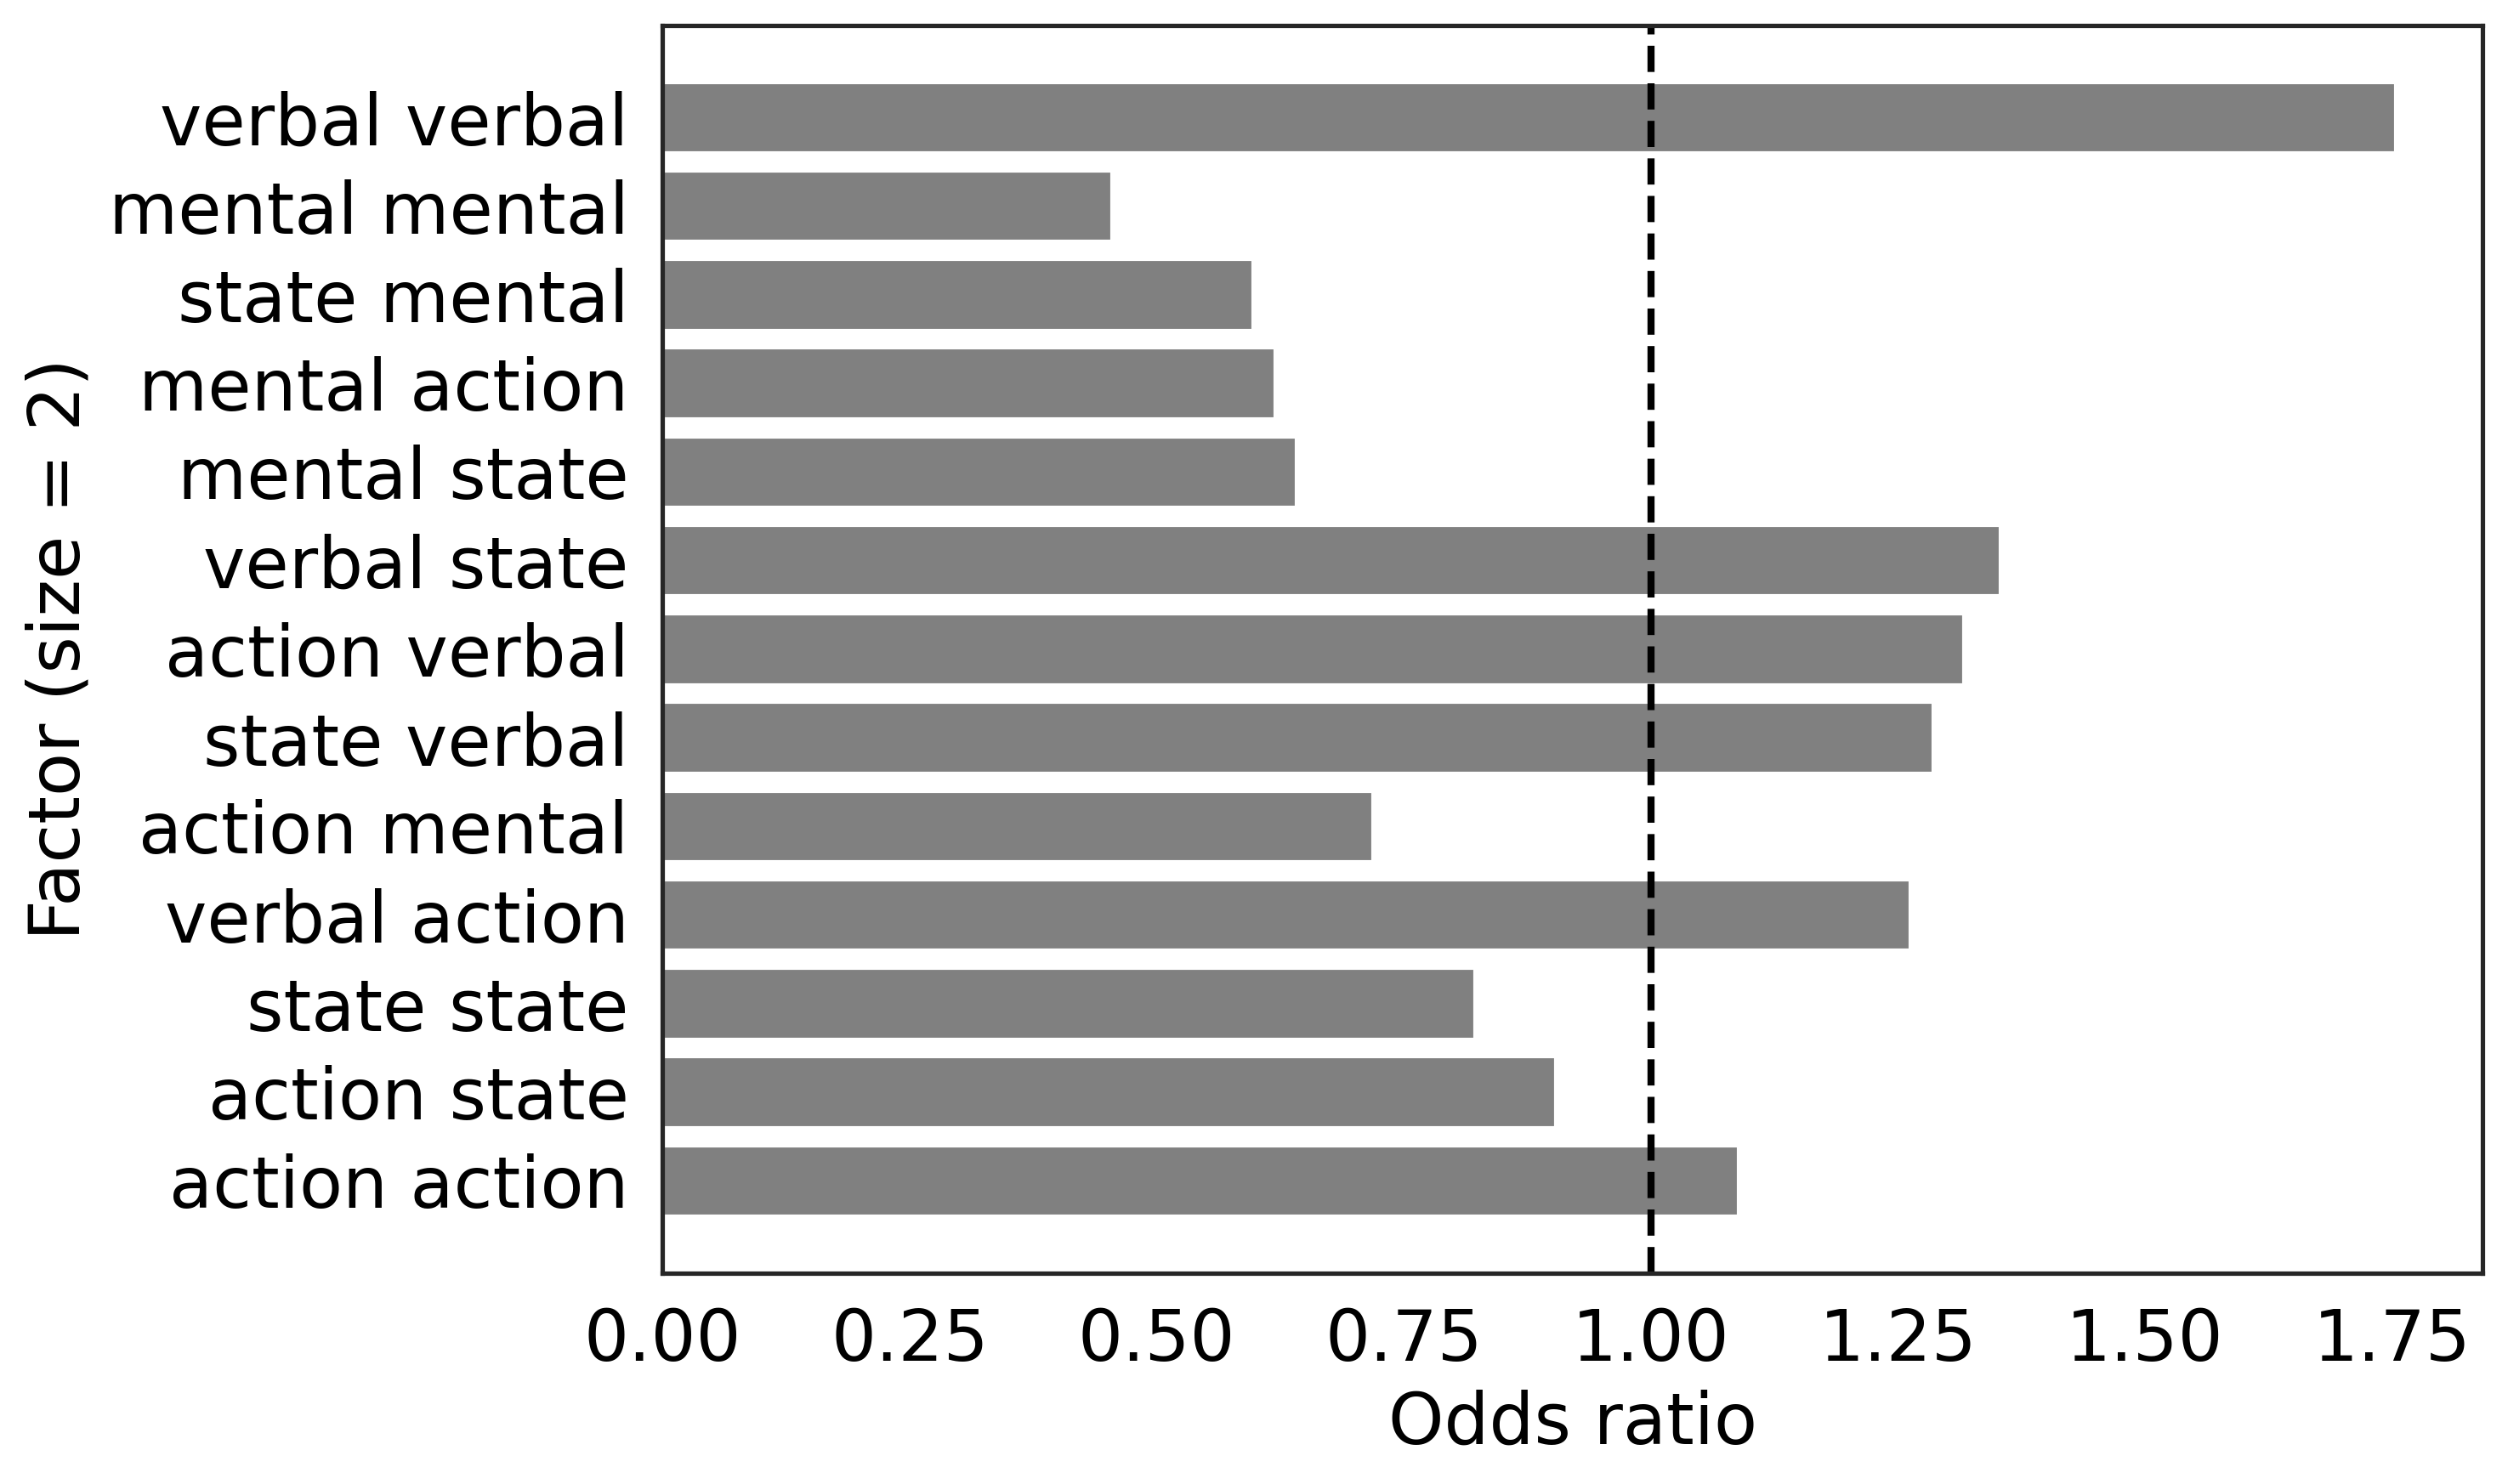
\includegraphics[scale=0.2]{img/viet_odds_2.png}
         \caption{Size 2.}
         \label{fig:viet_odds2}
     \end{subfigure}
         \begin{subfigure}[b]{0.4\textwidth}
         \centering
         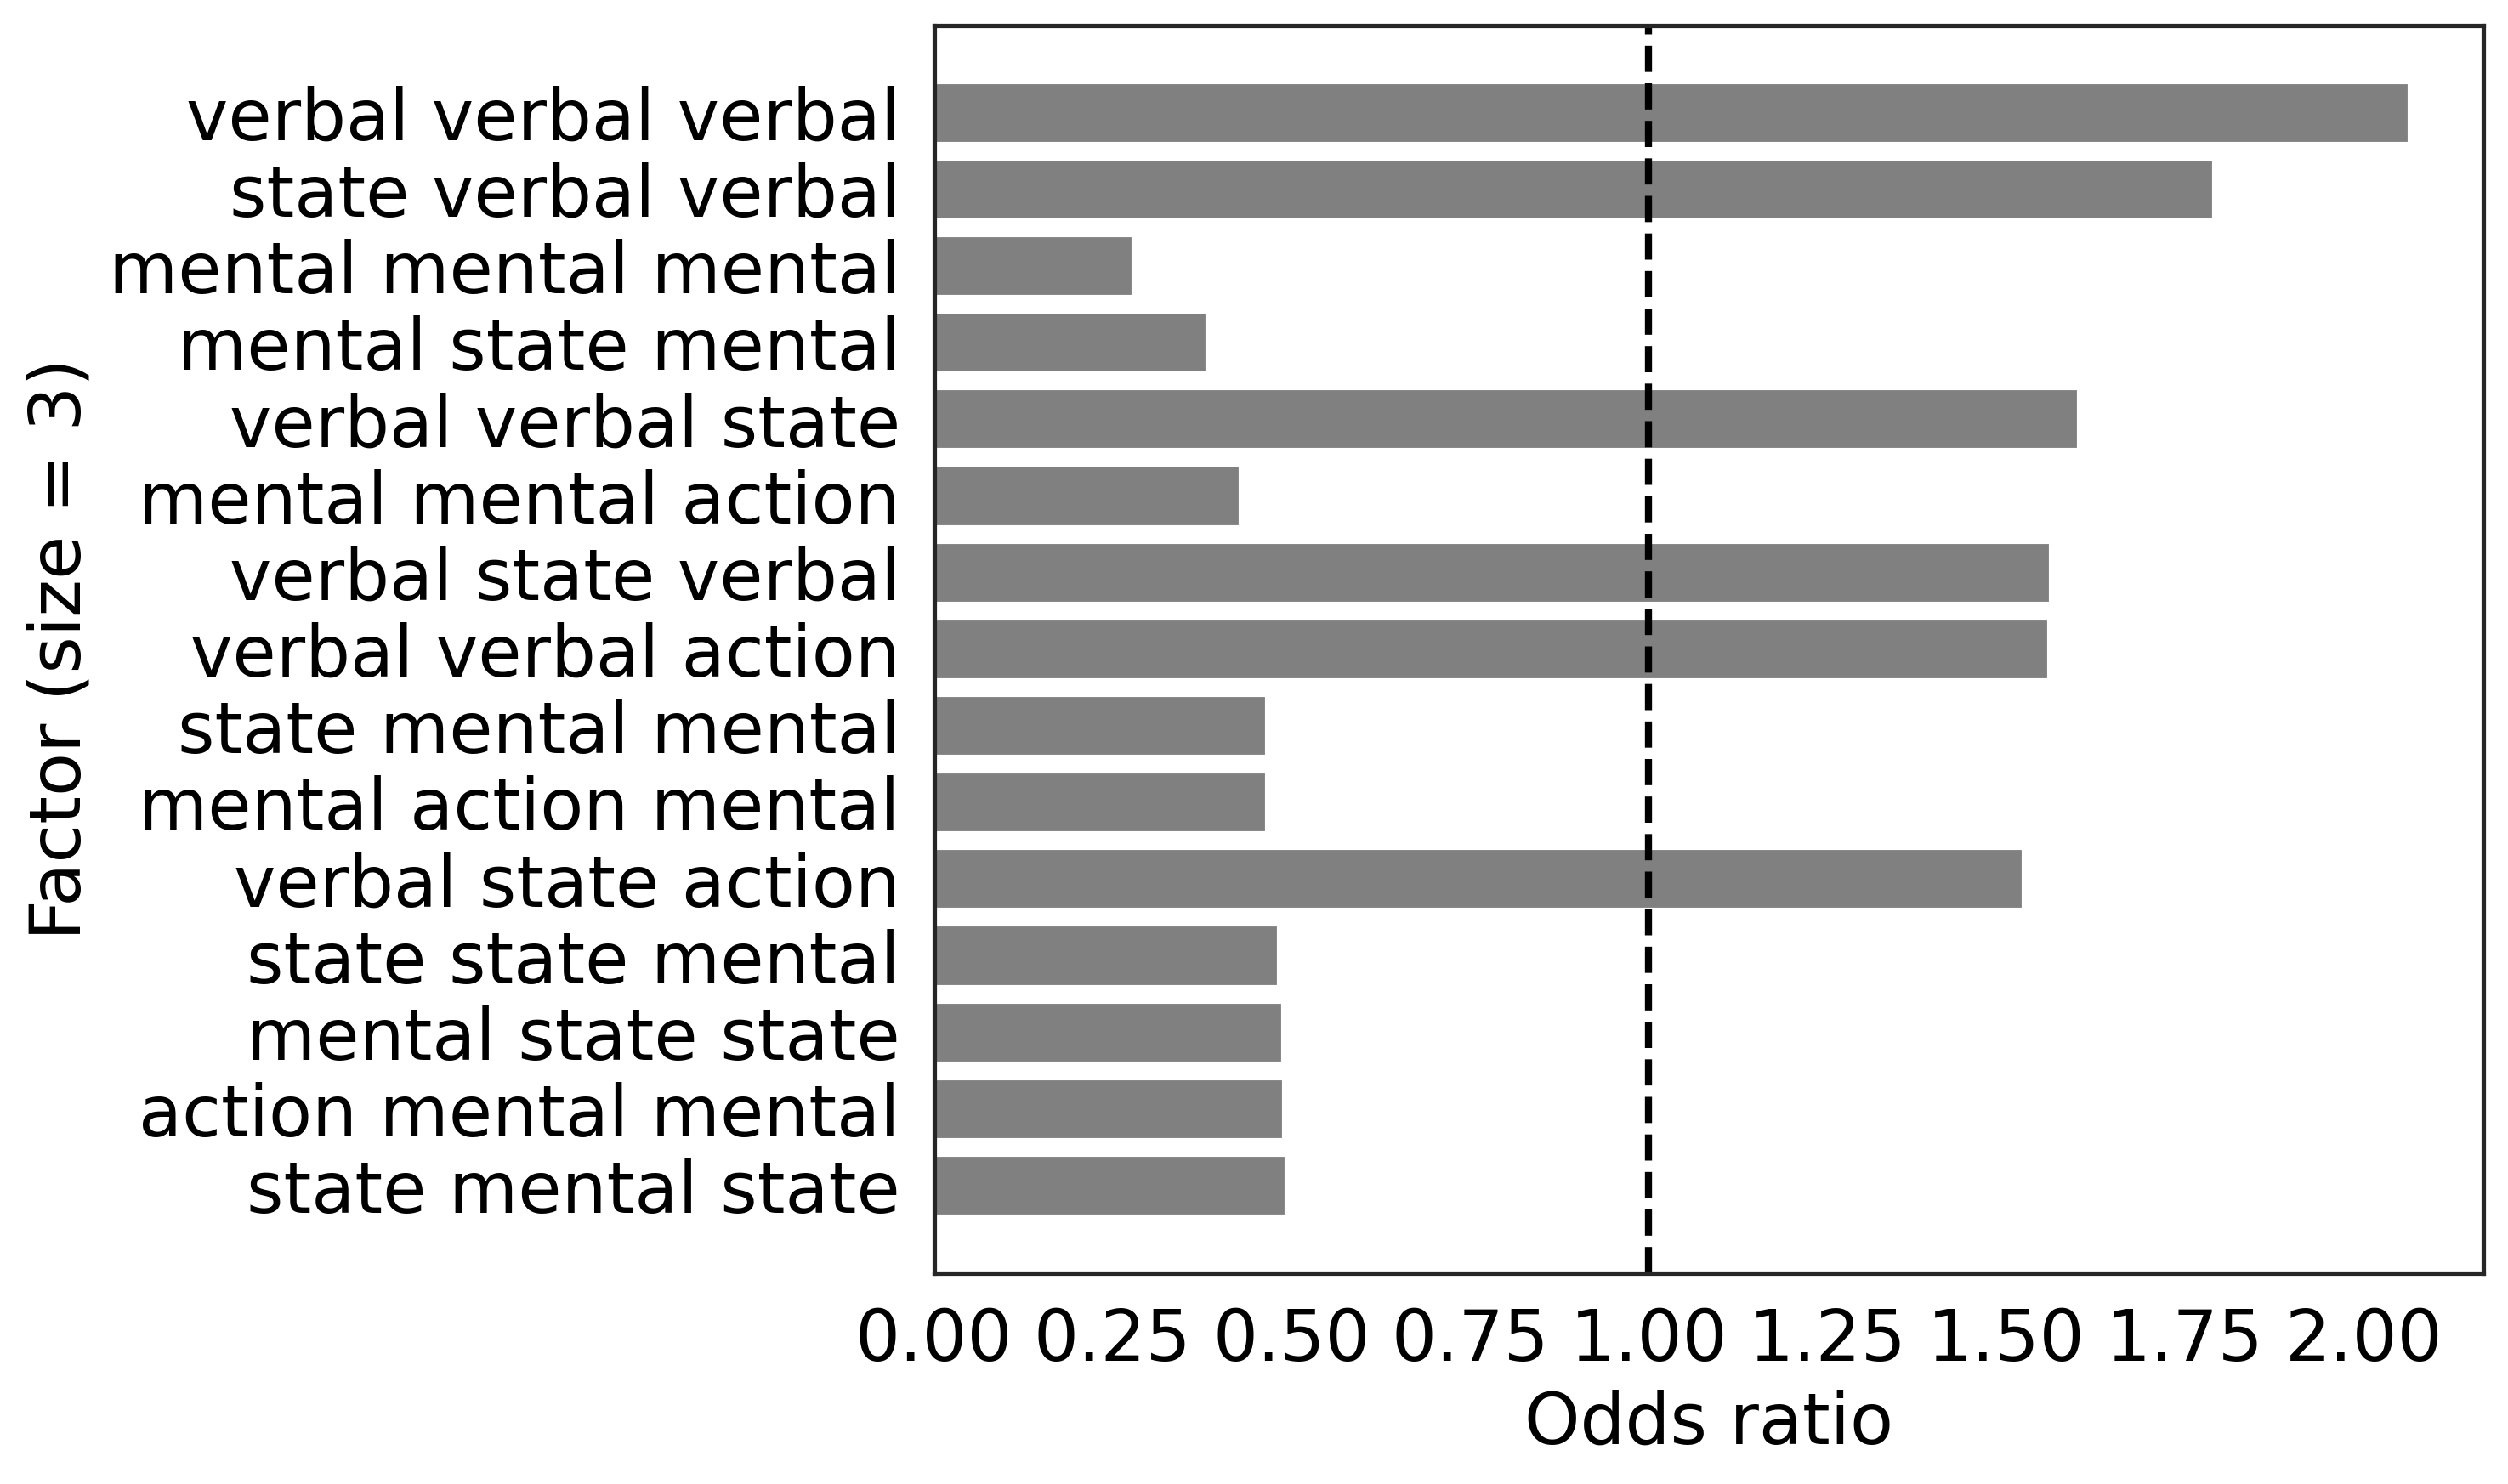
\includegraphics[scale=0.2]{img/viet_odds_3.png}
         \caption{Size 3.}
         \label{fig:viet_odds3}
     \end{subfigure}
        \caption{Top substring odds ratio between the veteran and the norm}
        \label{fig:viet_odds}
\end{figure}

\pause


We show a preference for \textit{viet} to remain in a verbal process, as indicated by substrings such as \textit{verbal.verbal} and \textit{verbal.verbal.verbal} with high odds ratios (respectively 2.00 and 1.75)

\end{frame}

\begin{frame}{Results on the Vietnam War veteran}

\begin{figure}
    \centering
    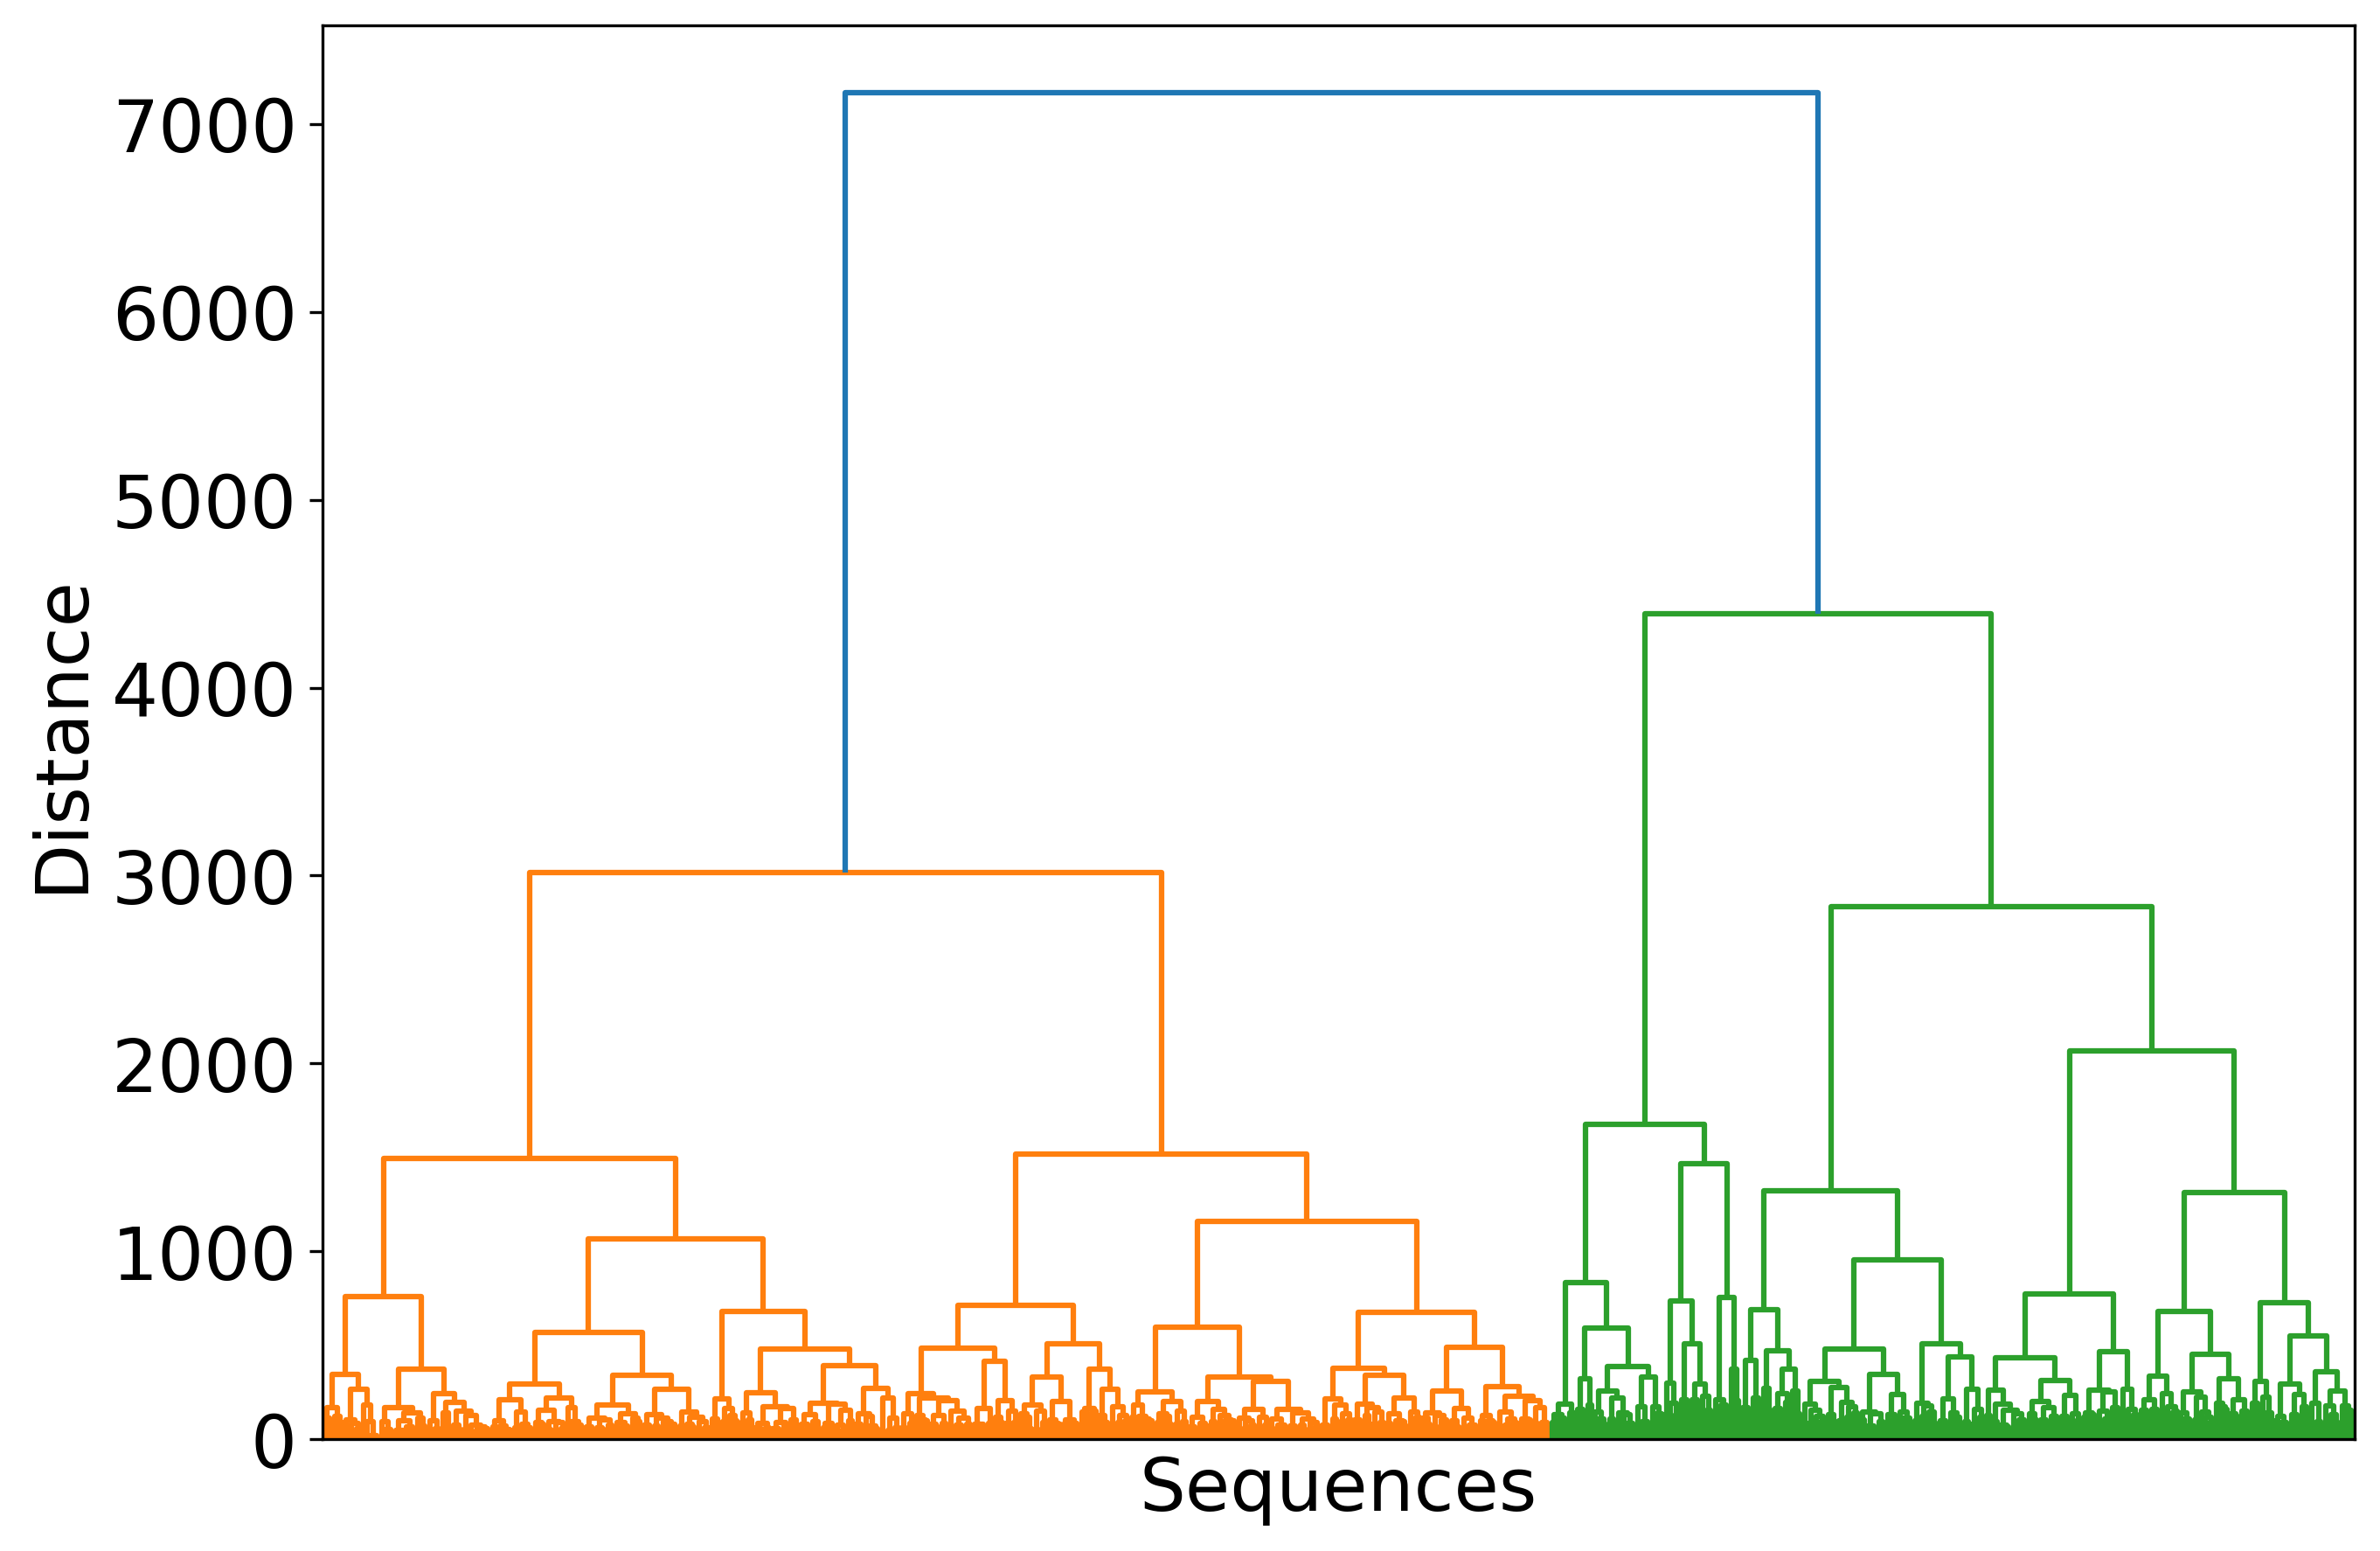
\includegraphics[width=0.55\linewidth]{img/dendogram_viet.png}
    \caption{Dendrogram with Ward linkage and cosine similarity}% on substrings of size one, two, and three.}
    \label{fig:dendogram}
\end{figure}

\vspace{0.25cm}
\pause

\textbf{Representative sequences}: \textit{savamasasaaamaaasavvvaaaaaaavssaaaaa} and \textit{sssssavaavssvsavvvvsmasasaasasaamaamvmsss} with $a=action, m=mental, s=state, v=verbal$

\vspace{0.25cm}
\pause

Two templates: a highly action-oriented structure or a more varied structure alternating between state and action processes
    
\end{frame}

\begin{frame}{Perspectives}

\begin{itemize}[<+->]
    \item \textbf{Authorship profiling}: identifying signature patterns (\textit{e.g.}, distinctive substrings) that characterize an author's unique way of constructing narratives
    \item \textbf{Style-conditioned narrative generation}: generating narratives from a sequence of linguistic features
    \item \textbf{Applying methods from complexity science and formal language theory}: analyzing subsequences, using complexity measures to quantify redundancies, etc.
\end{itemize}

\end{frame}

\begin{frame}{Conclusion}

\textbf{Research question}: How to model subjective experience in narratives?

\vspace{0.5cm}
\pause

\textbf{Steps}:

\begin{itemize}[<+->]
    \item Definition of objectives and scope using cognitive science
    \item Construction of an emotion dataset 
    \item Training of language models for emotion analysis 
    \item Formalization of style in narratives
\end{itemize}

\vspace{0.5cm}
%\pause

\small

\textit{My research models are publicly hosted on Hugging Face and were trained using the Jean Zay supercomputer}
    
\end{frame}

\begin{frame}{Pipeline for semantic clustering and description generation}

\begin{figure}
    \centering
    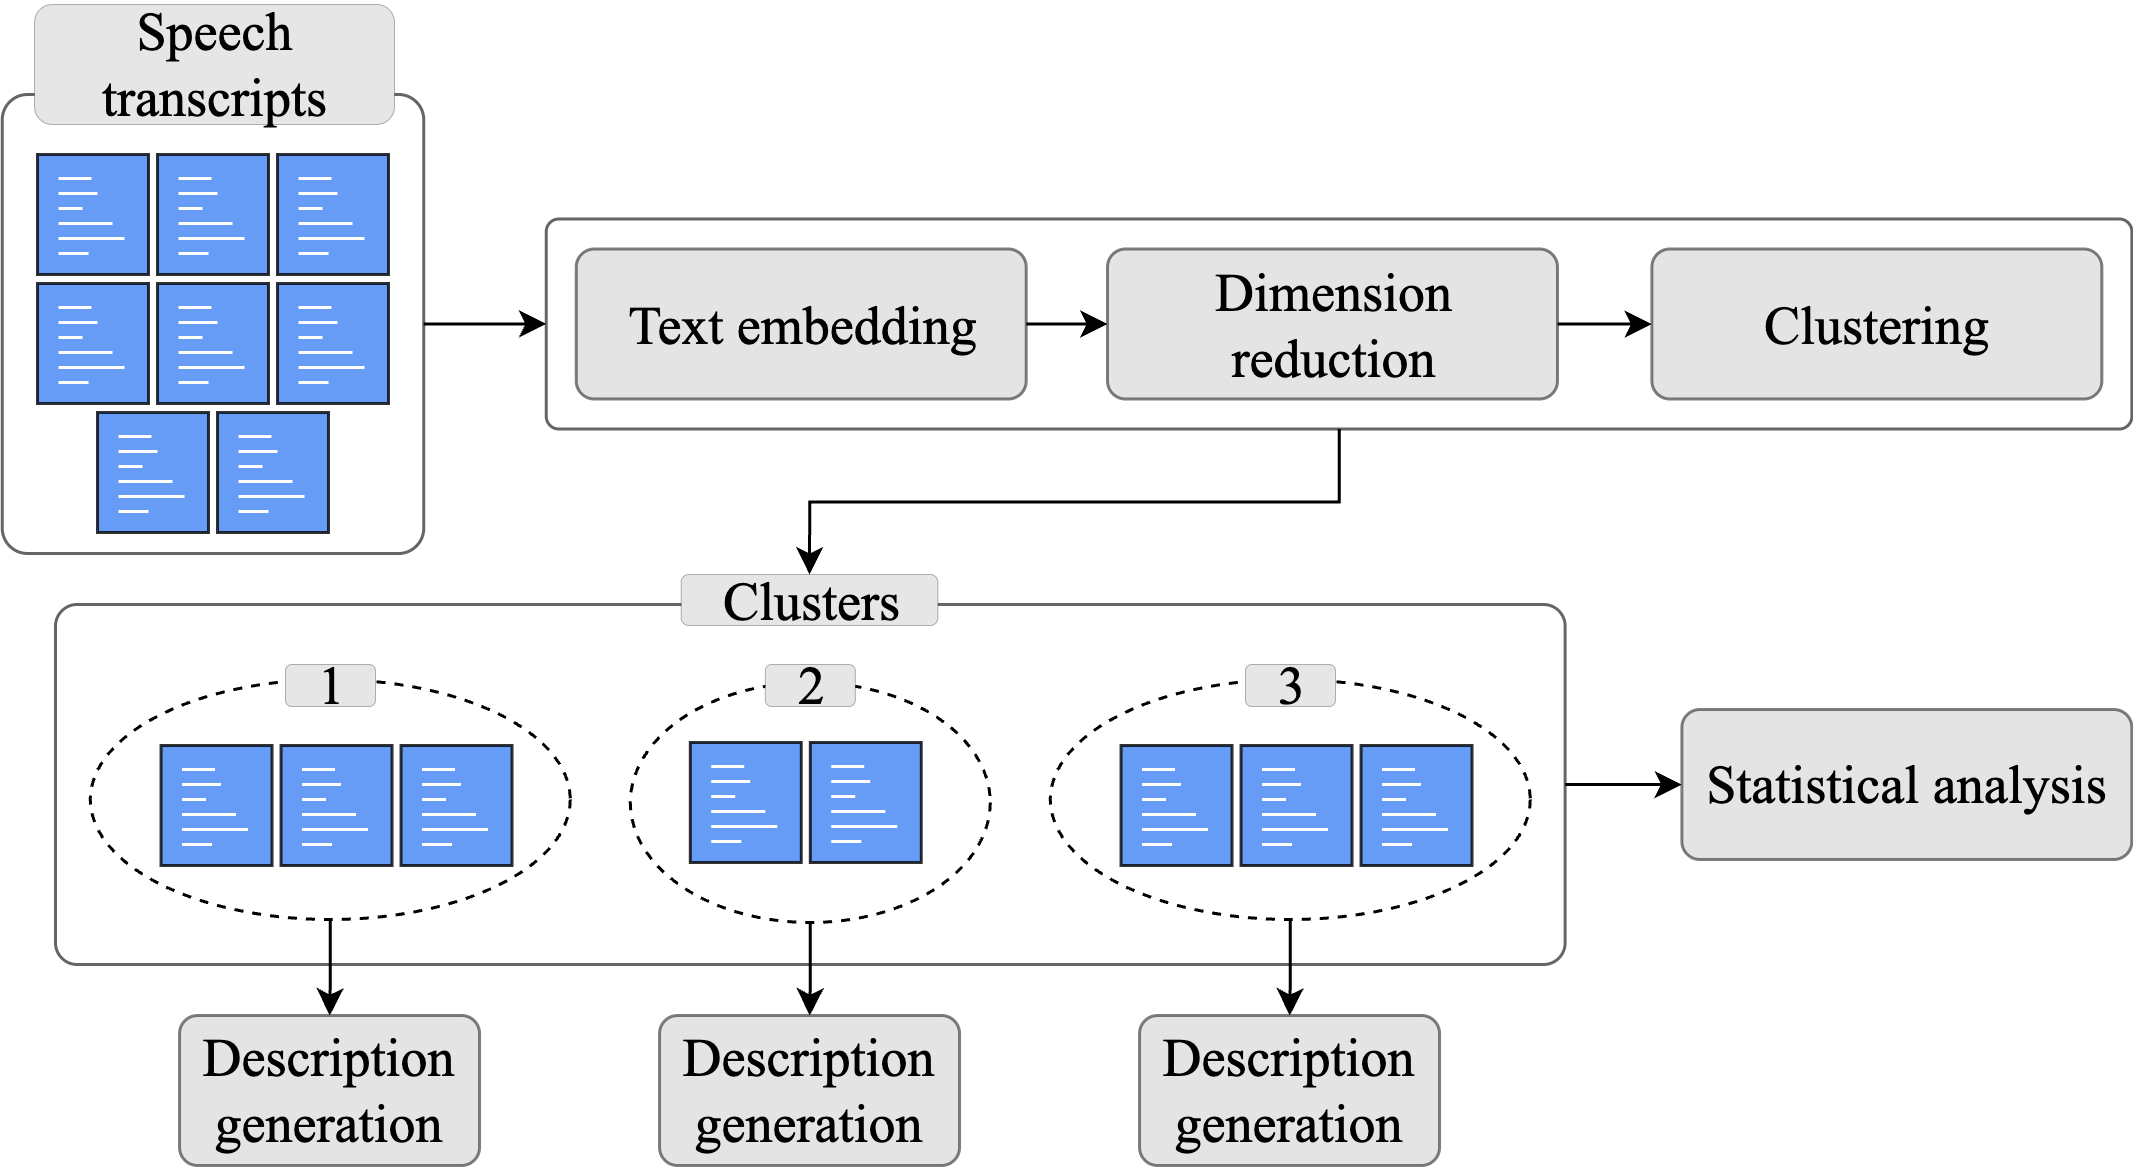
\includegraphics[scale=0.55]{img/topic_modeling/methods_v3.png}
    %\caption{\textbf{Computational pipeline for semantic clustering and description generation}. Speech transcripts are converted to semantic vectors via multilingual embeddings, dimensionally reduced, and grouped into clusters using density-based methods. Each cluster undergoes: (1) statistical analysis linking cluster membership to clinical/demographic  variables, and (2) automatic description generation where a large language model summarizes transcripts per cluster into human-readable natural language. This dual quantitative-qualitative output enables both statistical hypothesis testing and clinical interpretation of discovered topics.}
    %\caption{Each cluster undergoes: (1) statistical analysis linking cluster membership to clinical/demographic  variables, and (2) automatic description generation where a large language model summarizes transcripts per cluster into human-readable natural language.}
    \label{fig:methods}
\end{figure}

\end{frame}

\begin{frame}{Effect size across tasks and clinical scores}

\begin{figure}
    \centering
    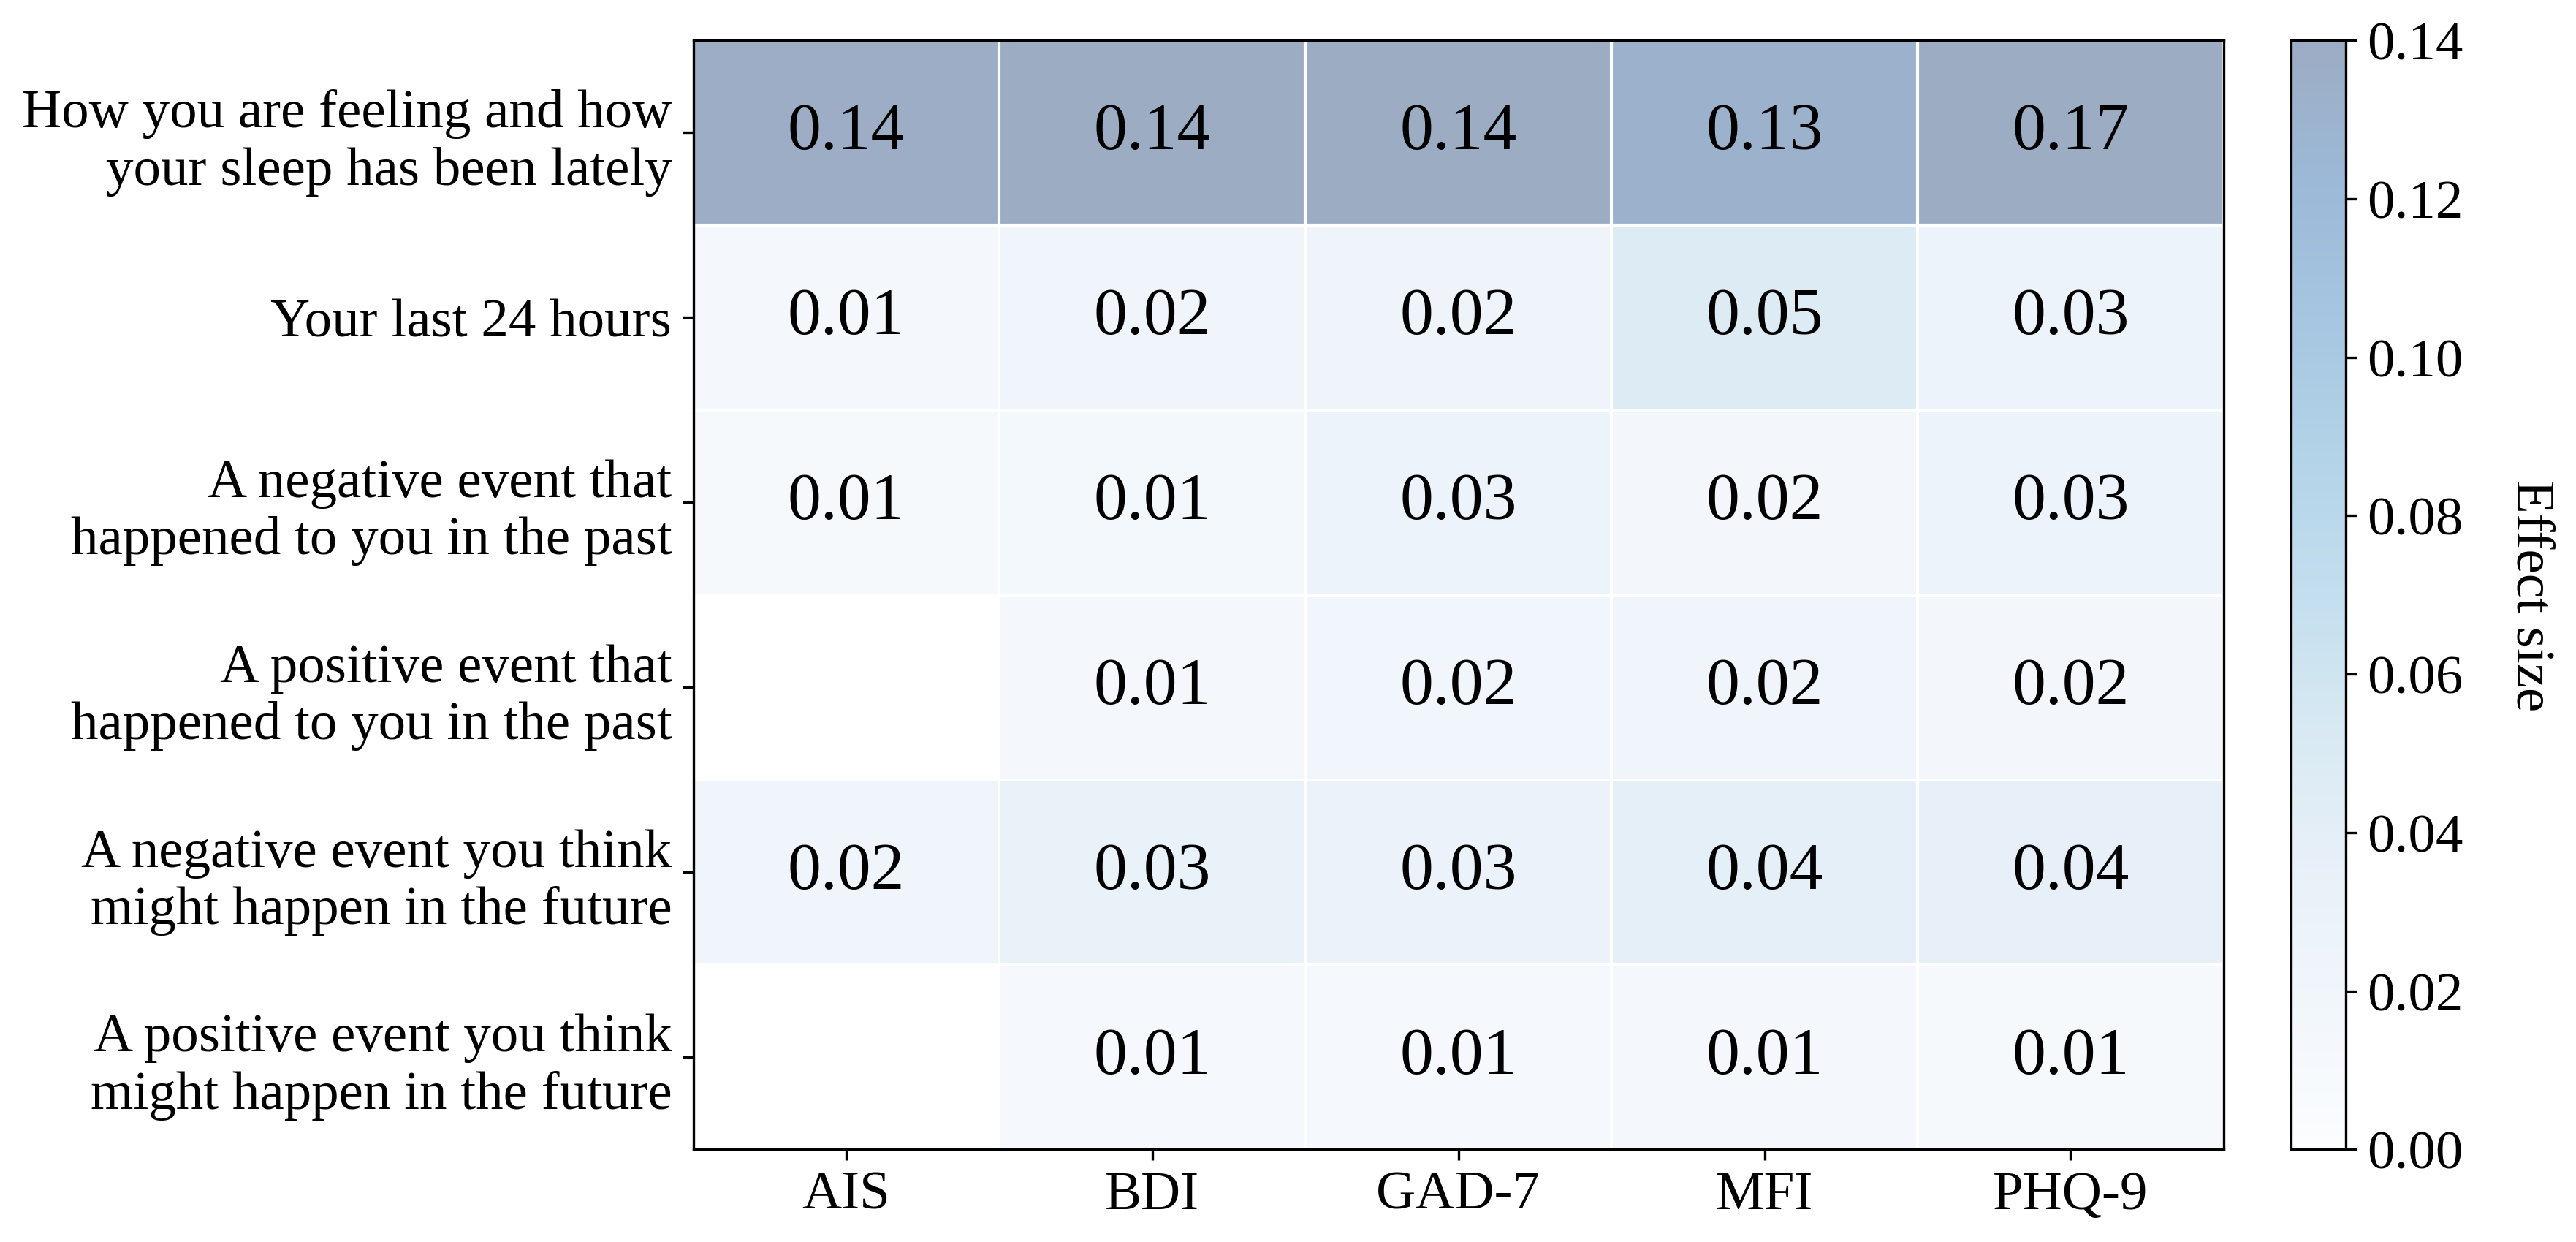
\includegraphics[scale=0.35]{img/topic_modeling/heatmap_effect_sizes/V5_V6_V7_V8_V9_V10_phq9_gad7_bdi_ais_mfi_global_heatmap.png}
    %\caption{Effect size across tasks and clinical scores for the French general population cohort}
    \label{fig:popgen_clinical_heatmap}
\end{figure}

\end{frame}

\begin{frame}{Effect size across tasks and demographics scores}

\begin{figure}
    \centering
    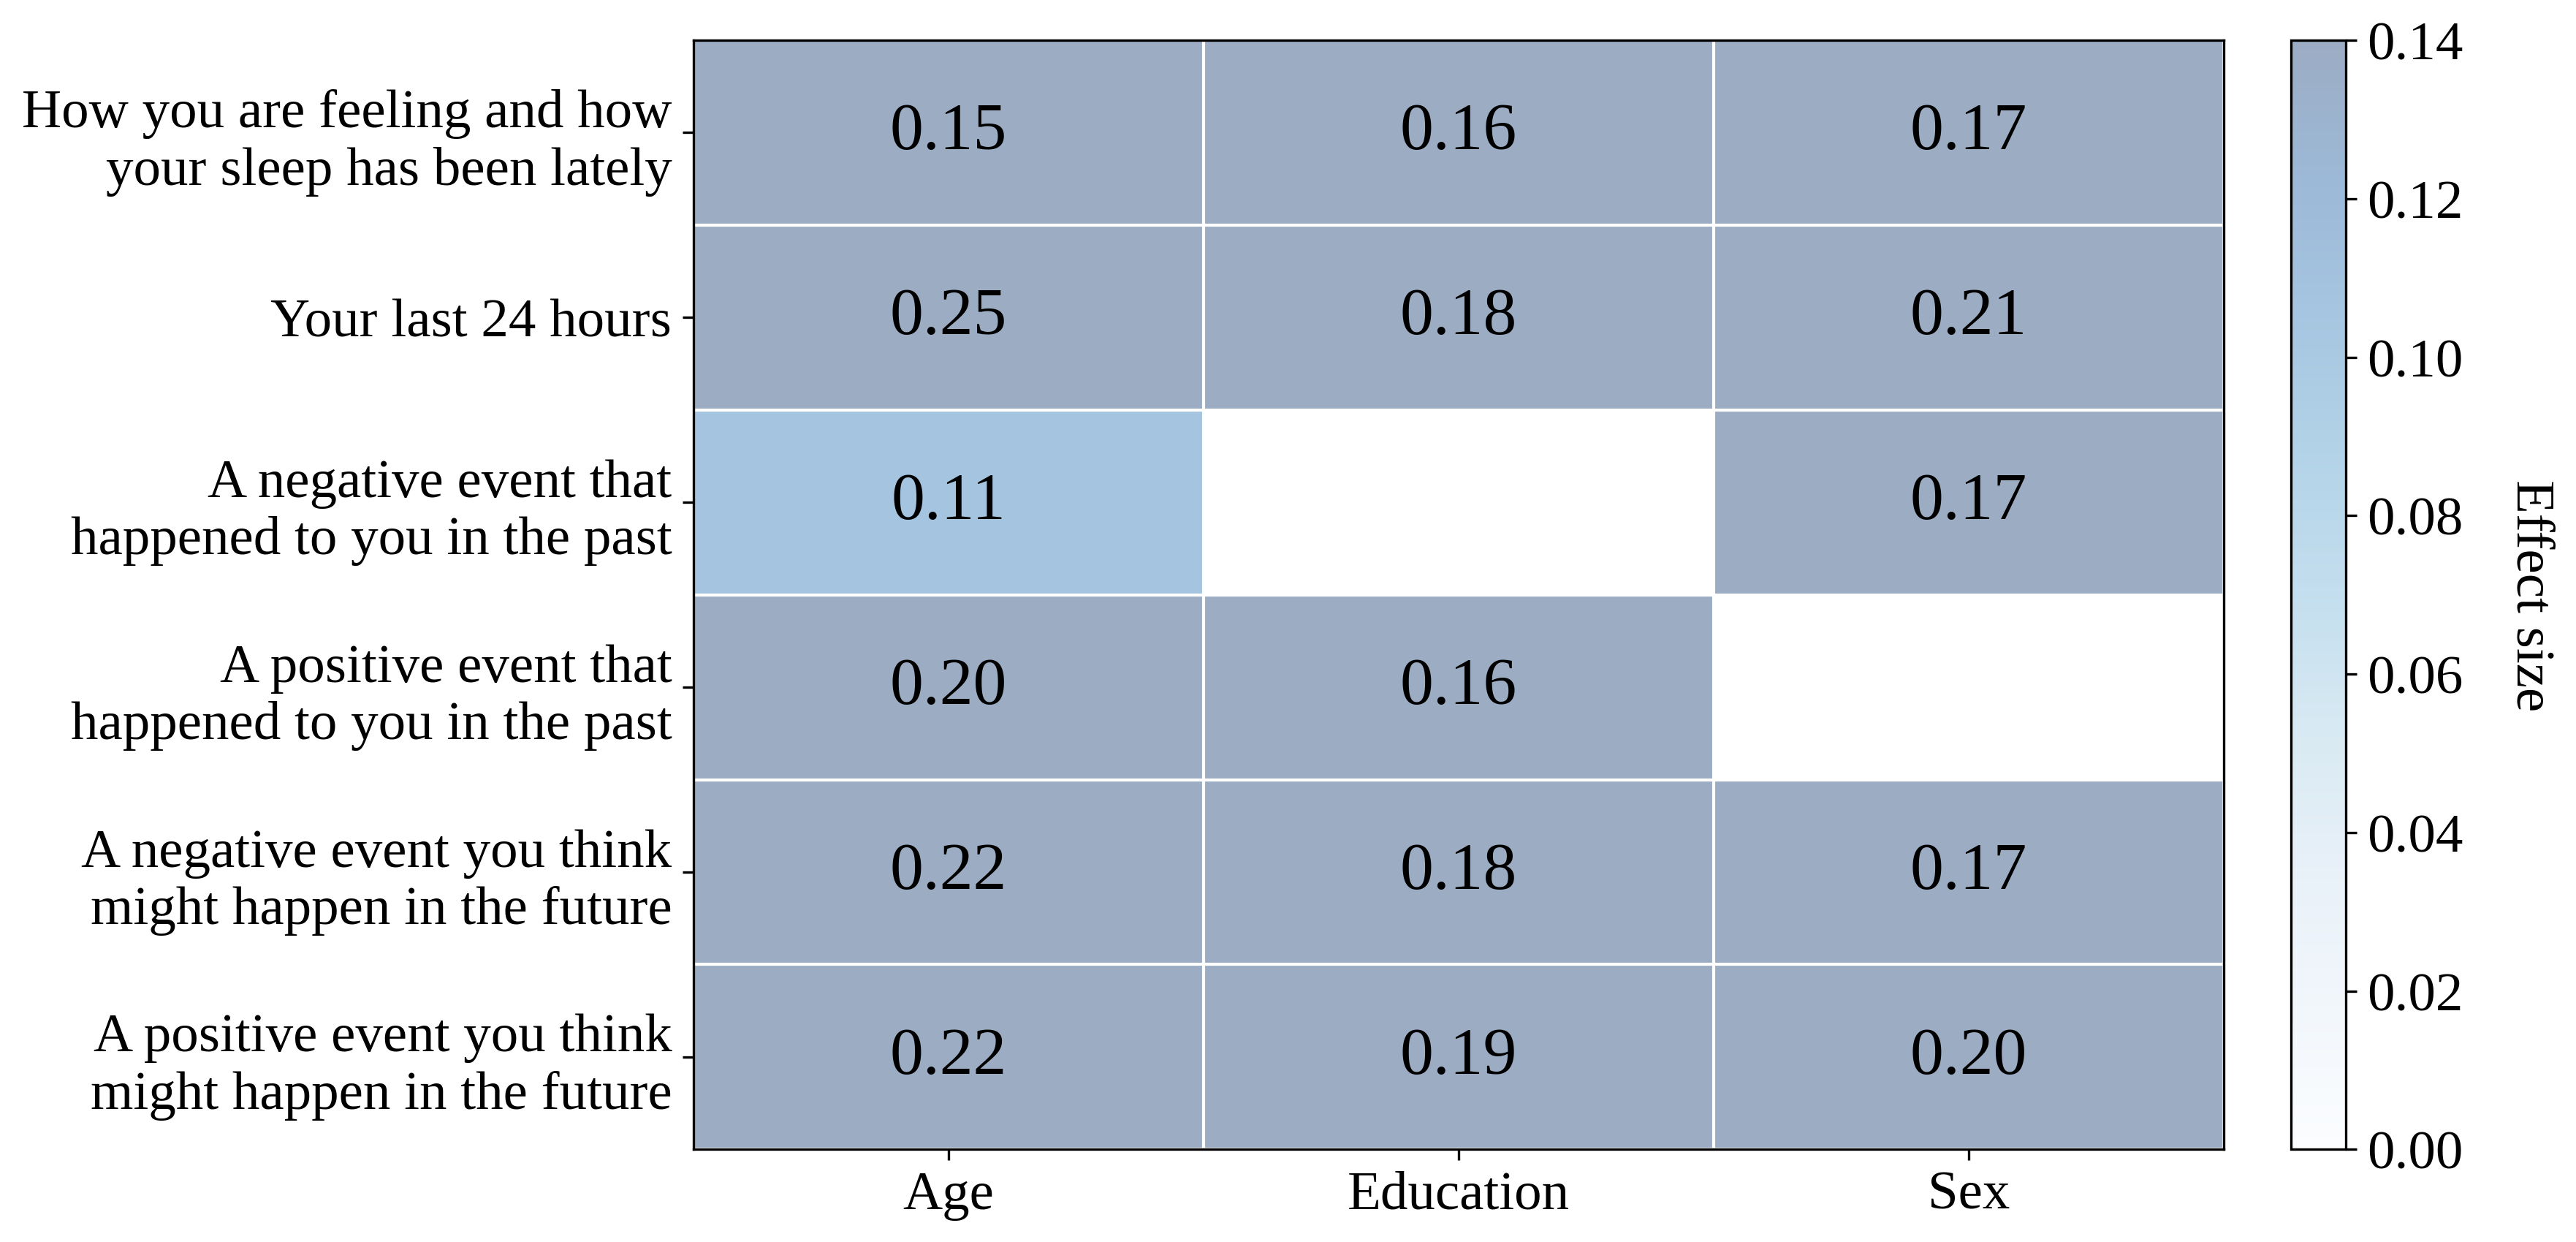
\includegraphics[scale=0.35]{img/topic_modeling/heatmap_effect_sizes/V5_V6_V7_V8_V9_V10_diploma_level_gender_age_global_heatmap.png}
    %\caption{Effect size across tasks and demographics scores for the French general population cohort}
    \label{fig:popgen_demo_heatmap}
\end{figure}

\end{frame}

\begin{frame}{Fine-grained mental health topic modeling}
  \begin{figure}
    \centering
    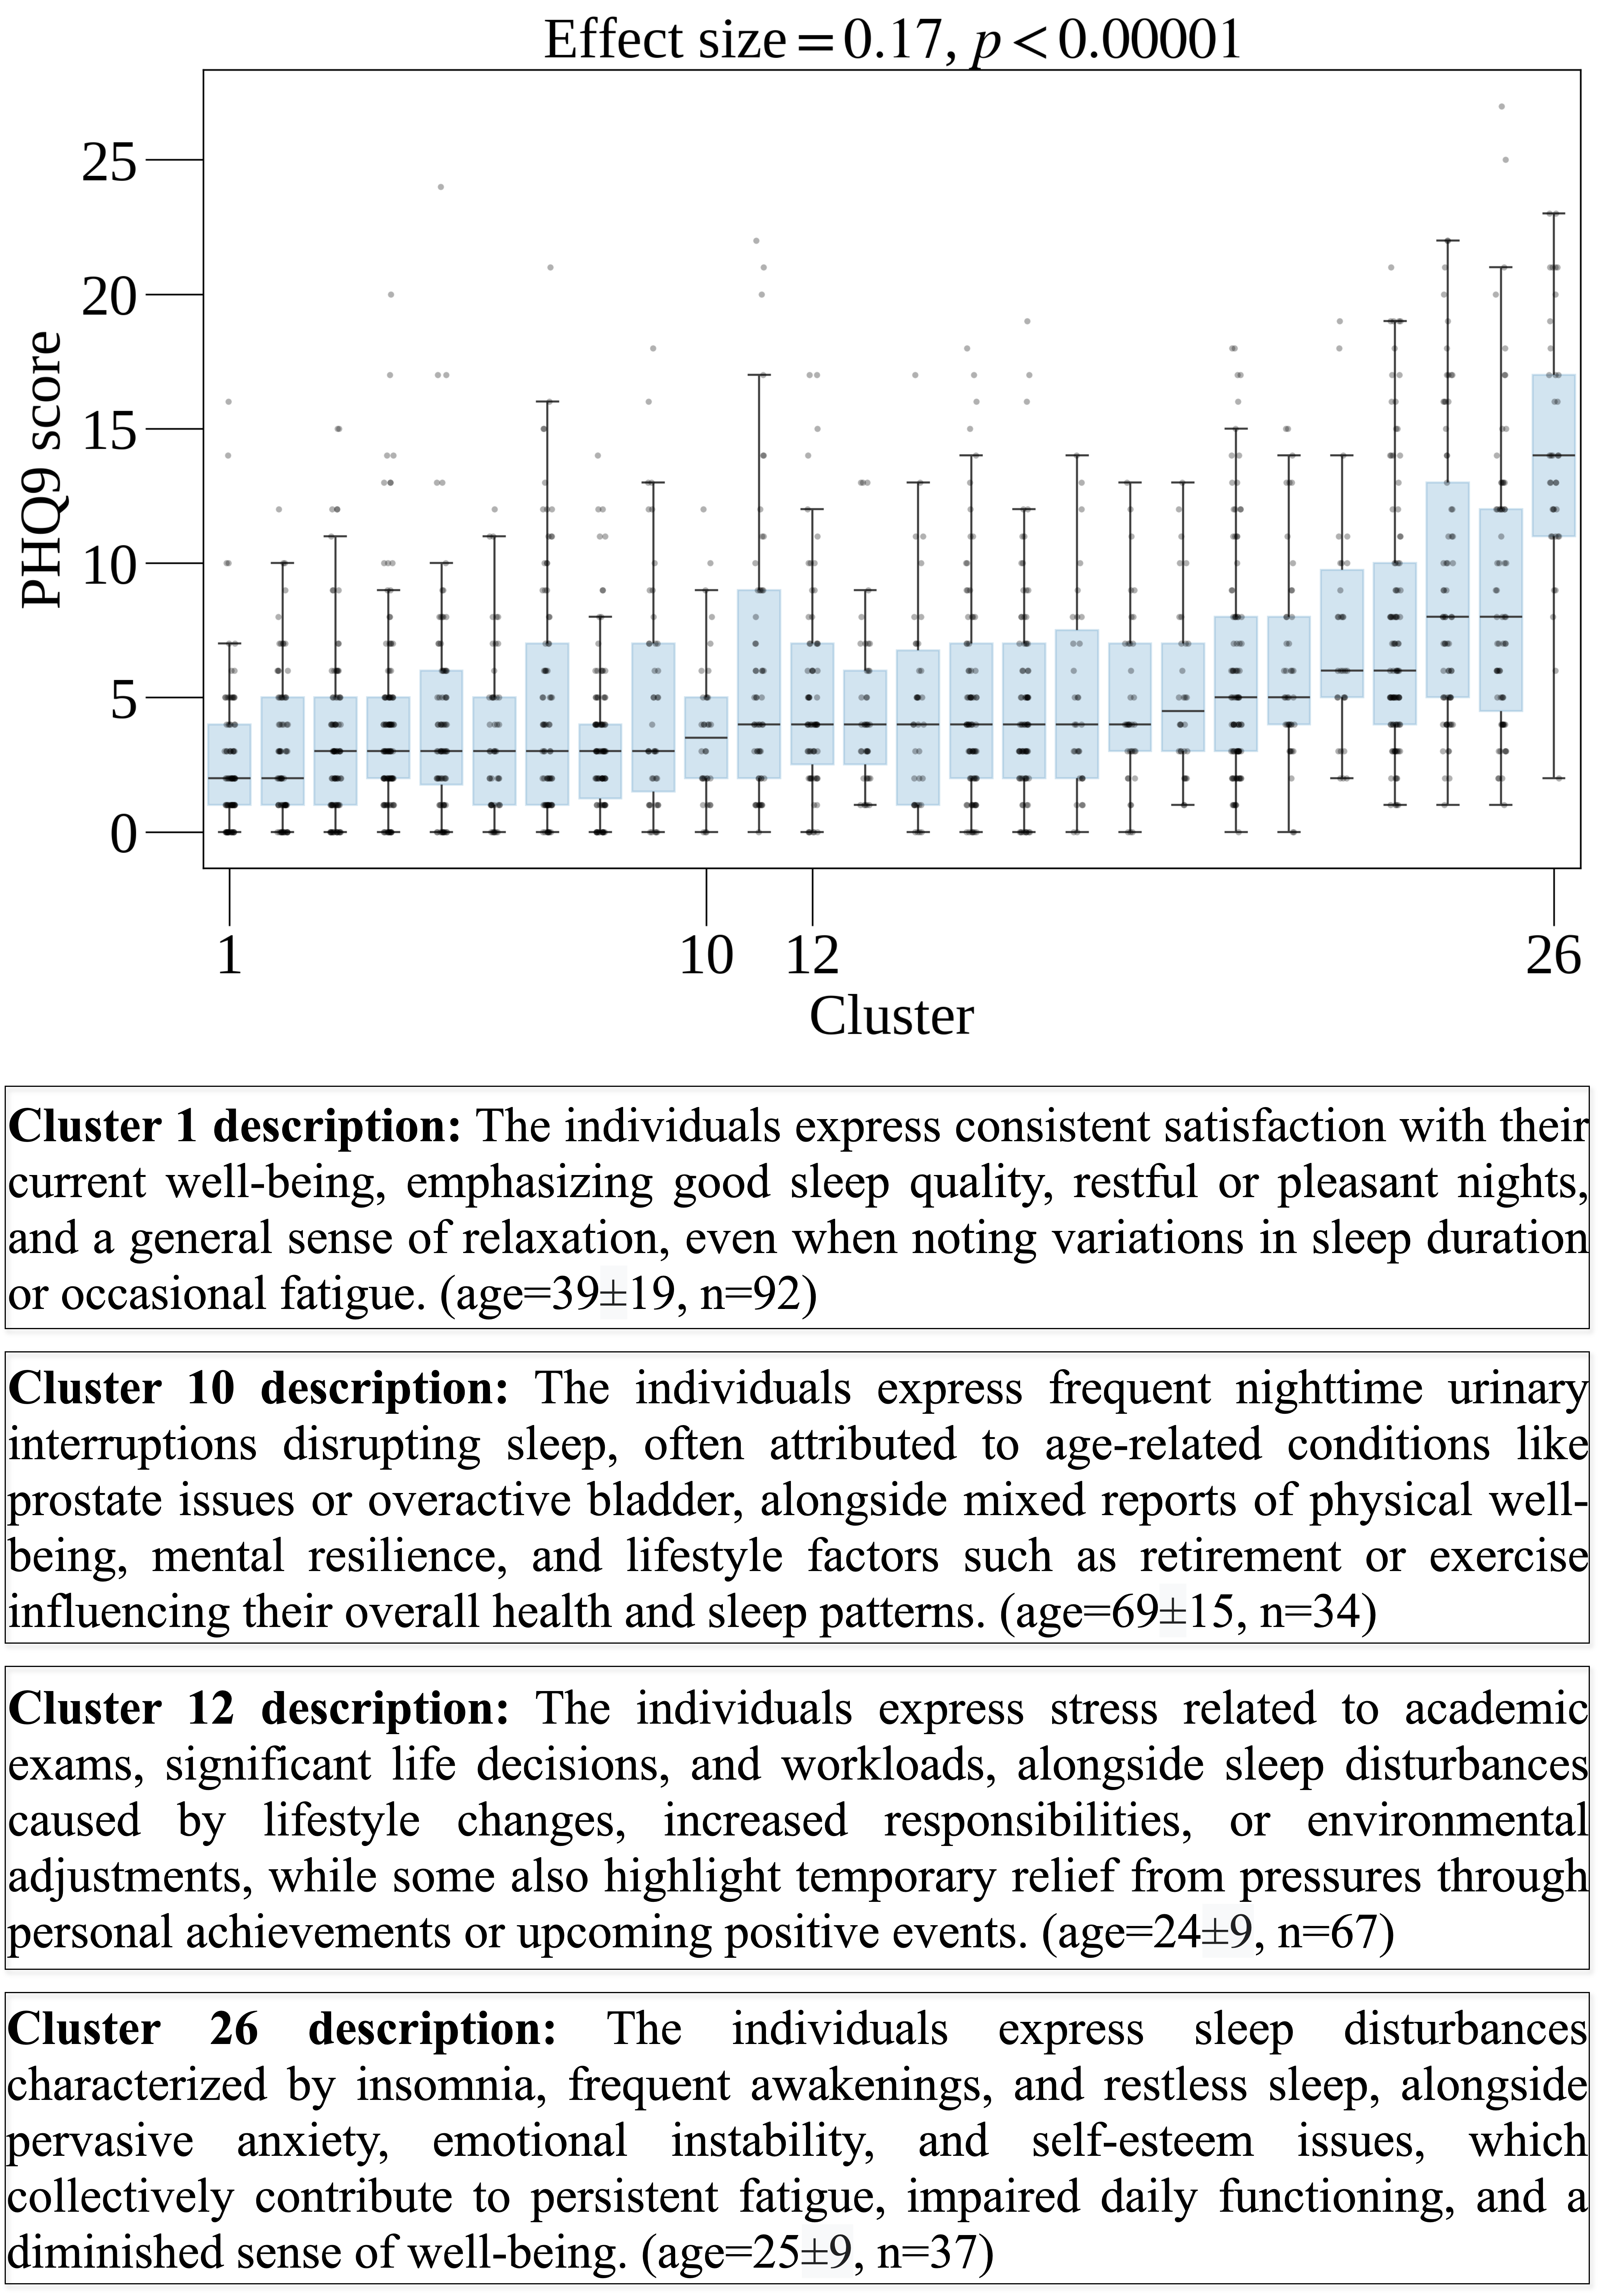
\includegraphics[scale=0.2]{img/topic_modeling/boxplot_description/popgen_description_larger.png}
    \caption{Distribution of PHQ-9 depression scores across automatically identified clusters in the French general population cohort (n=1,786 transcripts). Responses to the prompt 'Describe how you are feeling at the moment and how your sleep has been lately'. Box plots show median (center line), interquartile range (box), and 1.5x IQR whiskers. Effect size (Kruskal-Wallis H = 0.17, p < 0.00001) indicates moderate discrimination between clusters. Sample sizes per cluster range from n=34 to n=92. Selected cluster descriptions (Clusters 1, 10, 12, 26) were generated by Qwen3-14B summarizing 30 random transcripts per cluster.}
    \label{fig:popgen_description}
\end{figure}
\end{frame}

\begin{frame}{Appendix}

\begin{itemize}
    \item \textit{Fine-grained mental health topic modeling in different populations using large language models} (PhD internship, to be submitted for Nature Mental Health)
    \item \href{https://huggingface.co/gustavecortal/Piaget-8B}{Piaget}, a language model for psychological and philosophical reasoning, 2025.
    \item N. Richet, S. Belharbi, H. Aslam, M. Schadt, M. González-González, \textbf{G. Cortal}, A. Koerich, M. Pedersoli, A. Finkel, S. Bacon, E. Granger. \href{https://arxiv.org/abs/2407.12927}{Textualized and Feature-based Models for Compound Multimodal Emotion Recognition in the Wild}. \textit{ABAW, ECCV 2024}.
\end{itemize}
    
\end{frame}

\end{document}
